% ----------------------------------------------------------------
% AMS-LaTeX Paper ************************************************
% **** -----------------------------------------------------------
\documentclass[11pt]{amsart}
\usepackage{graphicx, mathabx, amssymb,amsfonts,amsmath,amsthm,newlfont}
\usepackage{epsfig,url}
\usepackage{enumerate,enumitem}
\usepackage[colorlinks=true,linkcolor=red,citecolor=blue]{hyperref}
\usepackage[dvipsnames]{xcolor}
\usepackage{color}

% !TEX root = ../Coherence.tex

%Clever ref
\usepackage[noabbrev,capitalize]{cleveref}


\usepackage[all,2cell]{xy} \UseAllTwocells \SilentMatrices


% ----------------------------------------------------------------
\vfuzz2pt % Don't report over-full v-boxes if over-edge is small
\hfuzz2pt % Don't report over-full h-boxes if over-edge is small
% THEOREMS -------------------------------------------------------
\newtheorem{thm}{Theorem}[section]
\newtheorem{corollary}[thm]{Corollary}
\newtheorem{lemmma}[thm]{Lemma}
\newtheorem{proposition}[thm]{Proposition}
\newtheorem{Questions}[thm]{Questions}
\theoremstyle{definition}
\newtheorem{definition}[thm]{Definition}

\newtheorem{conjectue}{Conjecture} 
\newtheorem{QQ}{Question} 
\newtheorem{prob}{Problem}
\newtheorem{ex}[thm]{Examples}
\newtheorem{example}[thm]{Example}
\newtheorem{policy}{Policy}
\theoremstyle{remark}
\newtheorem{rem}[thm]{Remark}
\newtheorem{caveat}[thm]{Caveat}
\numberwithin{equation}{section}
% MATH -----------------------------------------------------------
\newcommand{\norm}[1]{\left\Vert#1\right\Vert}
\newcommand{\abs}[1]{\left\vert#1\right\vert}
\newcommand{\set}[1]{\left\{#1\right\}}

\newcommand{\To}{\longrightarrow}
\newcommand*{\Longhookrightarrow}{\ensuremath{\lhook\joinrel\relbar\joinrel\rightarrow}}
\newcommand{\Z}{\mathbb Z}
\newcommand{\Q}{\mathbb Q}
\newcommand{\C}{\mathbb C}
\newcommand{\Ok}{\mathcal O}
\newcommand{\ai}{\mathfrak{a}}
\newcommand{\bi}{\mathfrak{b}}
\newcommand{\R}{\mathbb R}
\newcommand{\N}{\mathbb N}
\newcommand{\AM}{A}
\newcommand{\xx}{\mathsf{x}}
\newcommand{\eqv}{\mathrm{ev}}
\font \rus= wncyr10
\newcommand{\sha}{\, \hbox{\rus x} \,}

\newcommand{\Lie}{\mathrm{Lie}}

\newcommand{\GC}{\mathcal{GC}}
\newcommand{\q}{/\!/}

\newcommand{\tr}{\mathrm{tr}}
\newcommand{\id}{\mathrm{id}}

\newcommand{\can}{\mathrm{can}}

\newcommand{\mm}{\mathfrak{m}}

\newcommand{\GL}{\mathrm{GL}}
\newcommand{\LP}{L}
\newcommand{\FL}{F\!L}
\newcommand{\mc}{\mu}


\newcommand{\0}{\color{blue}{\mathsf{0}}}

%%%%Macros PL
\newcommand{\Alt}{ \mid\!\!\mid  } 
\newcommand{\inc}{\subseteq}
 \newcommand{\incs}{\subsetneq}
\newcommand{\union}{\cup}
\newcommand{\Union}{\bigcup}	
\newcommand{\comp}{\circ}
\newcommand{\setc}[2]{\set{#1 \mid #2}}

\newcommand \seq[2]{\shortstack{$#1$ \\ \mbox{}\\
                    \mbox{}\hrulefill\mbox{}\\ \mbox{}\\ $#2$}}
\newcommand{\cat}[1]{{\mathbb #1}}
\newcommand{\dl}{[\![} 			
\newcommand{\dr}{]\!]} 
\newcommand{\hyper}[1]{{\mathbb #1}}	
\newcommand{\restrH}[2]{\hyper{#1}\backslash #2}

%Operades

\def\calO{\mathcal{O}}
\newcommand{\KK}{\mathbb{K}}
\newcommand{\opd}[1]{\mathcal{#1}}

%Antischrieck
\newcommand{\as}{{\scriptstyle \text{\rm !`}}}

%Commentaires 

\newcommand{\Guillaume}[1]{\textcolor{magenta}{\underline{Guillaume}: #1}}

%Drapeau européen

\usepackage{graphicx,calc}
\newlength\myheight
\newlength\mydepth
\settototalheight\myheight{Xygp}
\settodepth\mydepth{Xygp}
\setlength\fboxsep{0pt}
\newcommand*\inlinegraphics[1]{%
  \settototalheight\myheight{Xygp}%
  \settodepth\mydepth{Xygp}%
  \raisebox{-\mydepth}{\includegraphics[height=\myheight]{#1}}%
}

%Dessins

\usepackage{tikz}
\usepackage{tikz-cd}
\usepackage{pgfplots}
\usepackage{pgfplotstable}
\tikzset{math3d/.style=
    {x= {(-0.353cm,-0.353cm)}, z={(0cm,1cm)},y={(1cm,0cm)}}}
\tikzset{JLL3d/.style=
    {x= {(0.4cm,-0.2cm)}, z={(0cm,1cm)},y={(-1cm,0cm)}}}
\usetikzlibrary{calc}
\usetikzlibrary{shapes,shapes.geometric,fit,positioning,calc,matrix}
\tikzset{
  optree/.style={scale=.5,thick,grow'=up,level distance=10mm,inner sep=1pt},
  comp/.style={draw=none,circle,fill,line width=0,inner sep=0pt},
  dot/.style={draw,circle,fill,inner sep=0pt,minimum width=3pt},
  circ/.style={draw,circle,inner sep=1pt,minimum width=4mm},
  emptycirc/.style={draw,circle,inner sep=1pt,minimum width=2mm},
  root/.style={level distance=10mm,inner sep=1pt},
  leaf/.style={draw=none,circle,fill,line width=0,inner sep=0pt},
  nodot/.style={draw,circle,inner sep=1pt},
}

\pgfplotsset{compat=1.12}



% ----------------------------------------------------------------

\def\abovespace{\vspace{12pt}}
\def\belowspace{\vspace{8pt}}



\addtolength{\hoffset}{-0.0in} \addtolength{\textwidth}{0in}
\addtolength{\voffset}{-0.0in} \addtolength{\textheight}{0.0in}


% -----------------------------------------------------------------

\title{Topological proofs of categorical coherence}

\author{Pierre-Louis Curien}
\address{IRIF, Universit\'e Paris Diderot and $\pi r^2$ team, Inria, France.}
\email{curien@irif.fr}

\author{Guillaume Laplante-Anfossi}
\address{School of Mathematics and Statistics, University of Melbourne, Victoria, Australia.}
\email{guillaume.laplanteanfossi@unimelb.edu.au}

\date{\today}

\subjclass[2010]{Primary 18F99} 

\keywords{Categorified operads, categorical coherence, Seifert--Van Kampen theorem, MacLane coherence theorem.}

\dedicatory{"We shall construct $KP_n$, as a CW-complex, in Section 2 and show that it is an $(n-1)$-ball. This gives an instant one-step proof of MacLane's theorem in full generality."  \\ --  Mikhail M. Kapranov}

%\thanks{The second author was supported by the European Union's Horizon 2020 research and innovation program under the Marie Sklodowska-Curie grant agreement No 754362 \inlinegraphics{EU.png}, by the Natural Sciences and Engineering Research Council of Canada (NSERC) and by the ANR-20-CE40-0016 Higher Algebra, Geometry and Topology.}


\begin{document}

\begin{abstract}
In this note, we give a short topological proof of coherence for categorified non-symmetric operads by using the fact that the diagrams involved are the 1-skeleton of simply connected CW complexes. 
In particular, we obtain a "one-step" topological proof of MacLane's coherence theorem, as suggested by Kapranov in 1993. 
In addition, we use Morse theory to give a second topological proof which is very close to MacLane's original argument. 
We use the same methods to deduce other categorical coherence results and discuss possible generalisations to higher categories. 
\end{abstract}

\maketitle

\setcounter{tocdepth}{1}
%\tableofcontents

% !TEX root = ../Coherence.tex

\section{Introduction} 
\label{s:introduction}




%%%%%%%%%%%%%%%%%%%%%%%%%%%%%%%%


\subsection{Coherence and rewriting for monoidal categories}

We start from a set $X$, considered as a set of  ``object variables"  (they are meant to be interpreted as objects in some category).  We define two sets   of object terms and morphism terms, respectively:
$$\begin{array}{l}
T::= x\  \;(\mbox{where}\;x\in X) \Alt I \Alt T\otimes T\\
M ::= \alpha \Alt \lambda \Alt\rho\Alt  \alpha^{-1} \Alt \lambda^{-1} \Alt\rho^{-1} \Alt M\comp M\Alt \id\Alt M\otimes M
\end{array}$$
In English, an object term is either a variable $x$, or $I$, or, if $s,t$ are object terms, then so is $(s\otimes t)$.
We actually only consider {\em well-typed} morphism terms  which are the ones accepted by the following typing rules, involving judgements of the form $M:T_1\rightarrow T_2$:
$$\seq{}{\alpha:(T_1\otimes T_2)\otimes T_3\rightarrow T_1\otimes(T_2\otimes T_3)}\quad\quad
\seq{}{\lambda:I\otimes T\rightarrow T}\quad\quad\seq{}{\rho:T\otimes I\rightarrow T}$$
$$\seq{}{\alpha^{-1}:T_1\otimes(T_2\otimes T_3)\rightarrow (T_1\otimes T_2)\otimes T_3}\quad\quad
\seq{}{\lambda^{-1}: T\rightarrow I\otimes T}\quad\quad\seq{}{\rho^{-1}:T\rightarrow T\otimes I}$$

$$\seq{}{\id:T\rightarrow T}\quad\quad \seq{M_1:T_1\rightarrow T_2\quad M_2:T_2\rightarrow T_3}{M_2\comp M_1:T_1\rightarrow T_3}\quad\quad \seq{M_1:T_1\rightarrow T'_1\quad M_2:T_2\rightarrow T'_2}{M_1\otimes M_2:T_1\otimes T_2\rightarrow T'_1\otimes T'_2}$$
In English, the formal typing rules read as: if all the typing assertions above the horizontal bar hold, then the typîng assertion below the bar holds.

One quotients the set of morphism terms by the laws of categories and of bifunctors, and by Mac Lane's coherence equations.
What one then obtains is the free monoidal category ${Free}(X)$ over $X$ i.e., for every {\em function} $\rho:X\rightarrow \cat{C}$ (mapping each $x$ to an object of  a monoidal category $\cat{C}$) there exists a unique strict monoidal functor $\dl \_\dr^\rho_{\cat{C}}:{Free}(X)\rightarrow\cat{C}$ that extends it.

The coherence theorem asserts that for any two terms $M,M':T\rightarrow T'$  of the {\em same type} we have $\dl M\dr^\rho_{\cat{C}}=\dl M'\dr^\rho_{\cat{C}}$  (for any monoidal category, and any valuation).

%%%%%%%%%%%%%%%%%%%%%%%%%%%%%%

\subsection{Categorified non-symmetric operads}

\begin{definition}[Categorified non-symmetric operad] A \emph{categorified non-symmetric operad} $\mathcal{P}$ is a collection $\left\{  \mathcal{P}(n)  \right\}_{n\in \mathbb{N}}$ of small categories equipped with bifunctors  
$$ \begin{array}{clll}
\circ_i&\colon& \mathcal{P}(n) \times
                  \mathcal{P}(k)
                  \longrightarrow \mathcal{P}(n+k-1) \ ,
                  & \text{for}\ 1 \leq i \leq n \ ,
\end{array}  $$
an object $\mathrm{id} \in \mathcal{P}(1)$ called \emph{unit}, and for each $\kappa \in \mathcal{P}(m)$,  $\mu \in \mathcal{P}(n)$, $\nu \in \mathcal{P}(k)$ natural isomorphisms 
$$ \begin{array}{clll}
    \beta_{\kappa,\mu,\nu}&\colon& 
    (\kappa \circ_i \mu) \circ_{j+i-1} \nu  \overset{\cong}{\longrightarrow} \kappa \circ_i (\mu \circ_j \nu) \ , &  \\
    \theta_{\kappa,\nu,\mu}&\colon& 
    (\kappa \circ_i \nu) \circ_{j+k-1} \mu 
    \overset{\cong}{\longrightarrow} (\kappa \circ_j \mu) \circ_i \nu \ , & \text{when}\ i < j \ , \\
    \lambda_\nu &\colon& 
    \mathrm{id} \circ_1 \nu \overset{\cong}{\longrightarrow} \nu \ , & \\
    \rho_\mu &\colon& 
    \mu \circ_i \mathrm{id} \overset{\cong}{\longrightarrow} \mu \ , & 
\end{array}  $$
such that the following diagrams commute: the triangle \\
\begin{center}
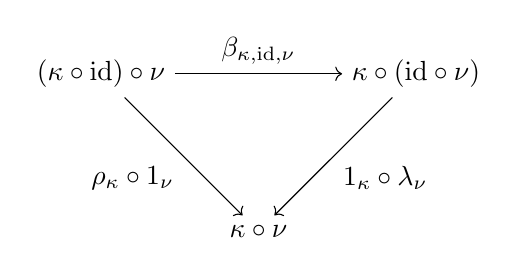
\begin{tikzpicture}[scale=2]
    \node (P1) at (-1,1) {$(\kappa \circ \mathrm{id})\circ \nu$};
    \node (P2) at (1,1) {$\kappa \circ (\mathrm{id}\circ \nu)$};
    \node (P3) at (0,0) {$\kappa \circ \nu$};
    \draw[->] (P1)--(P2) node[midway,above] {$\beta_{\kappa,\mathrm{id},\nu}$};
    \draw[->] (P1)--(P3) node[midway,below left] {$\rho_\kappa\circ 1_\nu$};
    \draw[->] (P2)--(P3) node[midway,below right] {$1_\kappa \circ \lambda_\nu$};
\end{tikzpicture} \quad \quad 
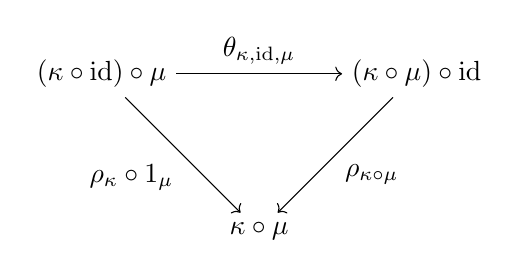
\begin{tikzpicture}[scale=2]
    \node (P1) at (-1,1) {$(\kappa \circ \mathrm{id})\circ \mu$};
    \node (P2) at (1,1) {$(\kappa\circ \mu)\circ\mathrm{id}$};
    \node (P3) at (0,0) {$\kappa \circ \mu$};
    \draw[->] (P1)--(P2) node[midway,above] {$\theta_{\kappa,\mathrm{id},\mu}$};
    \draw[->] (P1)--(P3) node[midway,below left] {$\rho_\kappa\circ 1_\mu$};
    \draw[->] (P2)--(P3) node[midway,below right] {$\rho_{\kappa\circ\mu}$};
\end{tikzpicture} \quad \ ,
\end{center}
pentagonal \\
\resizebox{\linewidth}{!}{
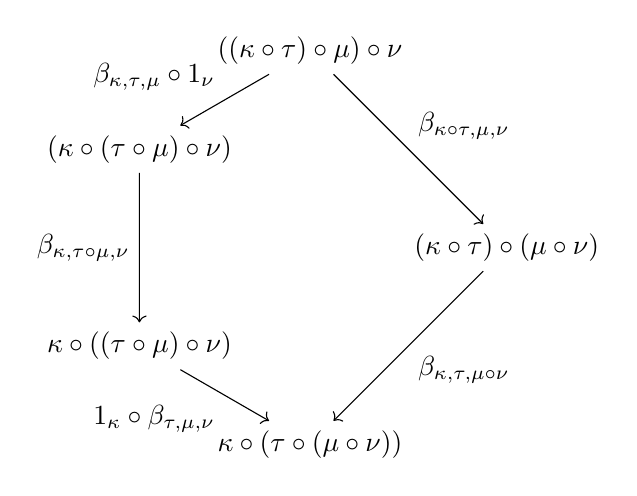
\begin{tikzpicture}[scale=2.5]
    \node (P1) at (0,1) {$((\kappa\circ\tau)\circ\mu)\circ\nu$};
    \node (P2) at (-0.866,0.5) {$(\kappa\circ(\tau\circ\mu)\circ\nu)$};
    \node (P3) at (-0.866,-0.5) {$\kappa\circ((\tau\circ\mu)\circ\nu)$};
    \node (P4) at (0,-1) {$\kappa\circ(\tau\circ(\mu\circ\nu))$};
    \node (P5) at (1,0) {$(\kappa\circ\tau)\circ(\mu\circ\nu)$} ;
    \draw[->] (P1)--(P2) node[midway,above left] {$\beta_{\kappa,\tau,\mu}\circ 1_\nu$};
    \draw[->] (P2)--(P3) node[midway,left] {$\beta_{\kappa,\tau\circ\mu,\nu}$};
    \draw[->] (P3)--(P4) node[midway,below left] {$1_\kappa \circ \beta_{\tau,\mu,\nu}$};
    \draw[->] (P1)--(P5) node[midway,above right] {$\beta_{\kappa\circ\tau,\mu,\nu}$};
    \draw[->] (P5)--(P4) node[midway,below right] {$\beta_{\kappa,\tau,\mu\circ\nu}$};
\end{tikzpicture} \quad 
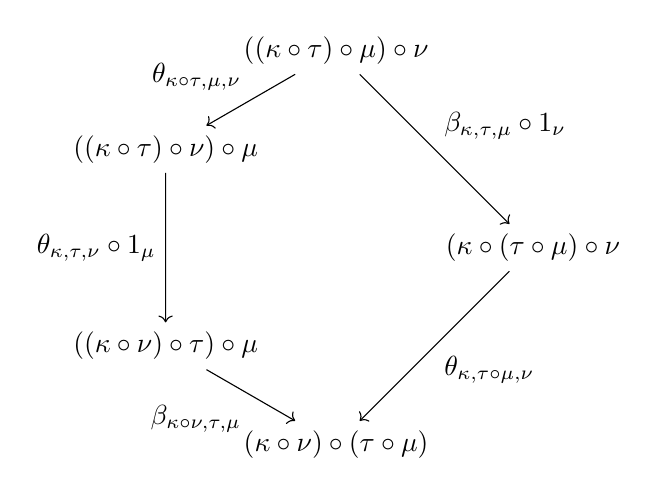
\begin{tikzpicture}[scale=2.5]
    \node (P1) at (0,1) {$((\kappa\circ\tau)\circ\mu)\circ\nu$};
    \node (P2) at (-0.866,0.5) {$((\kappa\circ\tau)\circ\nu)\circ\mu$};
    \node (P3) at (-0.866,-0.5) {$((\kappa\circ\nu)\circ\tau)\circ\mu$};
    \node (P4) at (0,-1) {$(\kappa\circ\nu)\circ(\tau\circ\mu)$};
    \node (P5) at (1,0) {$(\kappa\circ(\tau\circ\mu)\circ\nu$} ;
    \draw[->] (P1)--(P2) node[midway,above left] {$\theta_{\kappa\circ\tau,\mu,\nu}$};
    \draw[->] (P2)--(P3) node[midway,left] {$\theta_{\kappa,\tau,\nu}\circ 1_\mu$};
    \draw[->] (P3)--(P4) node[midway,below left] {$\beta_{\kappa\circ\nu,\tau,\mu}$};
    \draw[->] (P1)--(P5) node[midway,above right] {$\beta_{\kappa,\tau,\mu}\circ 1_\nu$};
    \draw[->] (P5)--(P4) node[midway,below right] {$\theta_{\kappa,\tau\circ\mu,\nu}$};
\end{tikzpicture} \quad 
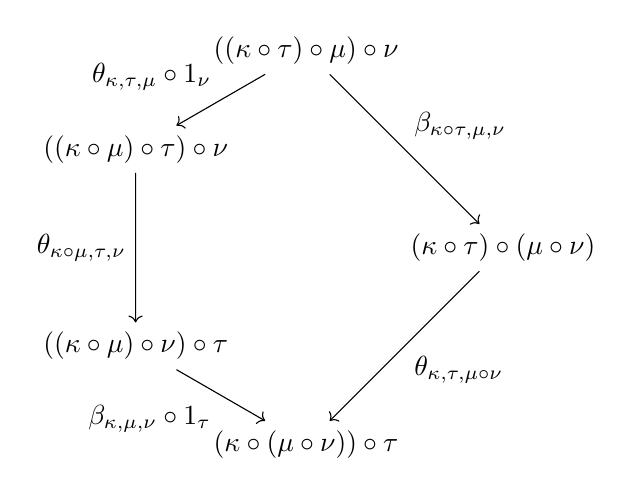
\begin{tikzpicture}[scale=2.5]
    \node (P1) at (0,1) {$((\kappa\circ\tau)\circ\mu)\circ\nu$};
    \node (P2) at (-0.866,0.5) {$((\kappa\circ\mu)\circ\tau)\circ\nu$};
    \node (P3) at (-0.866,-0.5) {$((\kappa\circ\mu)\circ\nu)\circ\tau$};
    \node (P4) at (0,-1) {$(\kappa\circ(\mu\circ\nu))\circ\tau$};
    \node (P5) at (1,0) {$(\kappa\circ\tau)\circ(\mu\circ\nu)$} ;
    \draw[->] (P1)--(P2) node[midway,above left] {$\theta_{\kappa,\tau,\mu}\circ 1_\nu$};
    \draw[->] (P2)--(P3) node[midway,left] {$\theta_{\kappa\circ\mu,\tau,\nu}$};
    \draw[->] (P3)--(P4) node[midway,below left] {$\beta_{\kappa,\mu,\nu}\circ 1_\tau$};
    \draw[->] (P1)--(P5) node[midway,above right] {$\beta_{\kappa\circ\tau,\mu,\nu}$};
    \draw[->] (P5)--(P4) node[midway,below right] {$\theta_{\kappa,\tau,\mu\circ\nu}$};
\end{tikzpicture} } \\
and hexagonal identities \\
\begin{center}
\resizebox{0.8\linewidth}{!}{
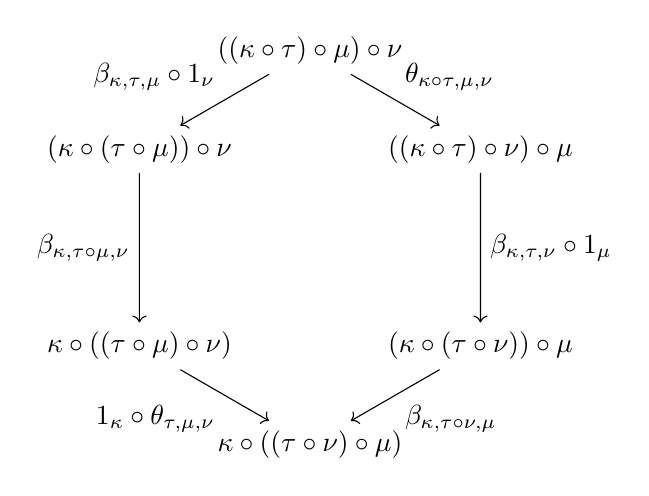
\begin{tikzpicture}[scale=2.5]
    \node (P1) at (0,1) {$((\kappa\circ\tau)\circ\mu)\circ\nu$};
    \node (P2) at (-0.866,0.5) {$(\kappa\circ(\tau\circ\mu))\circ\nu$};
    \node (P3) at (-0.866,-0.5) {$\kappa\circ((\tau\circ\mu)\circ\nu)$};
    \node (P4) at (0,-1) {$\kappa\circ((\tau\circ\nu)\circ\mu)$};
    \node (P5) at (0.866,0.5) {$((\kappa\circ\tau)\circ\nu)\circ\mu$} ;
    \node (P6) at (0.866,-0.5) {$(\kappa\circ(\tau\circ\nu))\circ\mu$};
    \draw[->] (P1)--(P2) node[midway,above left] {$\beta_{\kappa,\tau,\mu}\circ 1_\nu$};
    \draw[->] (P2)--(P3) node[midway,left] {$\beta_{\kappa,\tau\circ\mu,\nu}$};
    \draw[->] (P3)--(P4) node[midway,below left] {$1_\kappa \circ \theta_{\tau,\mu,\nu}$};
    \draw[->] (P1)--(P5) node[midway,above right] {$\theta_{\kappa\circ\tau,\mu,\nu}$};
    \draw[->] (P5)--(P6) node[midway,right] {$\beta_{\kappa,\tau,\nu}\circ 1_\mu$};
    \draw[->] (P6)--(P4) node[midway,below right] {$\beta_{\kappa,\tau\circ\nu,\mu}$};
\end{tikzpicture} \quad \quad
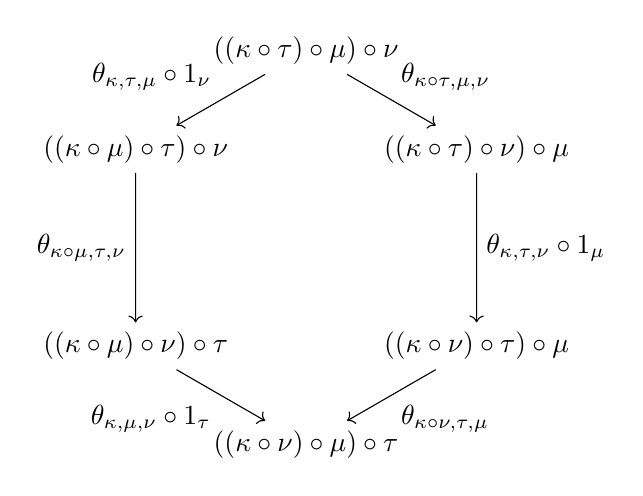
\begin{tikzpicture}[scale=2.5]
    \node (P1) at (0,1) {$((\kappa\circ\tau)\circ\mu)\circ\nu$};
    \node (P2) at (-0.866,0.5) {$((\kappa\circ\mu)\circ\tau)\circ\nu$};
    \node (P3) at (-0.866,-0.5) {$((\kappa\circ\mu)\circ\nu)\circ\tau$};
    \node (P4) at (0,-1) {$((\kappa\circ\nu)\circ\mu)\circ\tau$};
    \node (P5) at (0.866,0.5) {$((\kappa\circ\tau)\circ\nu)\circ\mu$} ;
    \node (P6) at (0.866,-0.5) {$((\kappa\circ\nu)\circ\tau)\circ\mu$};
    \draw[->] (P1)--(P2) node[midway,above left] {$\theta_{\kappa,\tau,\mu}\circ 1_\nu$};
    \draw[->] (P2)--(P3) node[midway,left] {$\theta_{\kappa\circ\mu,\tau,\nu}$};
    \draw[->] (P3)--(P4) node[midway,below left] {$\theta_{\kappa,\mu,\nu}\circ 1_\tau$};
    \draw[->] (P1)--(P5) node[midway,above right] {$\theta_{\kappa\circ\tau,\mu,\nu}$};
    \draw[->] (P5)--(P6) node[midway,right] {$\theta_{\kappa,\tau,\nu}\circ 1_\mu$};
    \draw[->] (P6)--(P4) node[midway,below right] {$\theta_{\kappa\circ\nu,\tau,\mu}$};
\end{tikzpicture}  } \quad \ .
\end{center}
\end{definition}

A categorified ns operad concentrated in arity 1 is a monoidal category.


%%%%%%%%%%%%%%%%%%%%%%%%%%%%%%%%%%%%%%%%


\subsection{Basic facts about polytopes}

Vertex figure
Every pair of edges is connected by a path

\subsection{Reminders on hypergraph polytopes}

A hypergraph is given by a set  $H$ of vertices (the carrier), and a subset 
$\hyper{H}\inc {\mathcal{P}}(H)\backslash\emptyset$ such that $\Union \hyper{H}=H$.
 The elements of $\hyper{H}$ are called the {\em hyperedges} of $\hyper{H}$.  
 We always assume that $\hyper{H}$ is {\em atomic}, by which we mean that 
 $\set{x}\in \hyper{H}$, for all $x\in H$. 
 Identifying $x$ with $\set{x}$, $H$ can be seen as the set of  hyperedges of 
 cardinality $1$, also called {\em vertices}. We shall use the convention to 
 give the same name to the hypergraph and to its carrier, in different fonts. 
 %When this convention cannot be used, we use the notation $V(\hyper{H})$ for the set of vertices of $\hyper{H}$.
% In the sequel, we shall write $\hyper{H}$ for an atomic  hypergraph, and $H$ for its set of vertices, i.e. 
%$H=\Union\hyper{H}$.
A hyperedge of cardinality 2 is called an {\em edge}.  Note that any ordinary graph $(V,E)$ can be viewed as the atomic hypergraph
$\setc{\set{v}}{v\in V} \union \setc{e}{e\in E}$ (with no hyperedges of cardinality $\geq 3$). 

\smallskip
 
If $\hyper{H}$ is a hypergraph,  and if  $X\inc H$, we set
$\hyper{H}_X:=\setc{Z}{Z\in \hyper{H}\;\mbox{and}\; Z\inc X}$, and $\restrH{H}{X}=\hyper{H}_{H\backslash X}$.
We say that $\hyper{H}$ is {\em connected} if there is no non-trivial partition $H=X_1\union X_2$ such that $\hyper{H}=\hyper{H}_{X_1}\union \hyper{H}_{X_2}$, and that $X\inc H$ is connected in $\hyper{H}$ if $\hyper{H}_X$ is connected.
%All our hypergraphs will be finite. 
For each finite hypergraph there exists a partition
$H=X_1\union\ldots\union X_m$ such that each $\hyper{H}_{X_i}$ is connected and $\hyper{H}=\Union(\hyper{H}_{X_i})$.  The $\hyper{H}_{X_i}$'s are  the {\em connected components} of $\hyper{H}$. The notation
$\hyper{H},X  \leadsto \hyper{H}_1,\ldots, \hyper{H}_n$
 will mean that  $\hyper{H}_1,\ldots,\hyper{H}_n$ are  the
 connected components of $\restrH{H}{X}$.  
%We shall  write
%$\hyper{H}_i$  for
%$\hyper{H}_{H_i}$. 

\smallskip

Do\v sen and Petri\'c~\cite{DP} have proposed the following insightful reading of the data of a finite connected hypergraph $\hyper{H}$ as a truncated simplex: the elements of $H$ are identified with the facets (i.e. codimension 1 faces) of the $(|H|-1)$-dimensional simplex, and each $\emptyset\incs X\incs H$, $|X|\geq 2$, such that    $\hyper{H}_X$ is connected designates the intersection of the facets in $X$ as a face to be truncated.
The obtained polytopes, called \emph{hypergraph polytopes}, extend the construction of graph associahedra \cite{CD-CCGA, Zel06}, and are equivalent to nestohedra, as introduced by Postnikov \cite{P09}.  Moreover,  the faces of the   polytope obtained by performing  all the prescribed truncations  are labeled by non-planar trees whose nodes are decorated by non-empty subsets of $H$, called {\em constructs}, whose recursive definition  we give next using a syntax introduced in \cite{COI}:

\smallskip
Let  $\emptyset\neq Y\subseteq H$. If   $\hyper{H},Y  \leadsto \hyper{H}_1,\ldots, \hyper{H}_n$, and if  $T_1,\ldots,T_n$ are constructs of $\hyper{H}_1,\ldots,\hyper{H}_n$, respectively, then the tree obtained by grafting $T_1,\ldots,T_n$ on the root node decorated by $Y$, denoted by $Y(T_1,\ldots,T_n)$, is a construct of  $\hyper{H}$~\footnote{\label{construct-tubing} Constructs are in one-to-one correspondence with tubings as defined in \cite{CD-CCGA}: for a given construct $T$, each tube of the associated tubing is given by a node of $T$ and all its descendance. There are  as many tubes in the tubing as nodes in the construct.}. We write $Y=\mbox{root}(Y(T_1,\ldots,T_n))$.

\smallskip
 The base case is when $Y=H$ (and hence $n=0$): then the one-node tree $H()$ (written simply $H$) is a construct.
We write $T:\hyper{H}$ to denote that $T$ is a construct of $\hyper{H}$. 
The formalism of constructs   allows us to view the inclusion of faces of a hypergraph polytope through the process of contracting tree edges: by contracting an edge of a construct and  merging the decorations of the two nodes related by that edge, one gets a covering construct.

\smallskip
Simplices are ``encoded'' as the hypergraphs  $$\hyper{S}^X=\setc{\set{x}}{x\in X}\union\set{\set{X}}$$ (no truncation prescribed). The constructs have the form $Y(\ldots,\set{y},\ldots)$ where $\emptyset\incs Y\inc X$ and $y$ ranges over $H\backslash Y$, and are therefore isomorphic to multipointed sets. In order to illustrate  how the hypergraph structure dictates truncations, consider the hypergraph $\hyper{H}=\set{\set{x},\set{y},\set{z},\set{y,z}, \set{x,y,z}}$, obtained from $\hyper{S}^{\{x,y,z\}}$ by adding the edge $\{y,z\}$. The construct 
 $\set{x}(\set{y},\set{z}):\hyper{S}^{\{x,y,z\}}$ is {\em not} a construct of $\hyper{H}$, since $\hyper{H}_{\set{y,z}}$ is connected.  Instead, $\hyper{H}$ features 3 new constructs: 
$\set{x}(\set{y}(\set{z}))$, $\set{x}(\set{z}(\set{y}))$ and $\set{x}(\set{y,z})$, encoding two  vertices and one edge, obtained by truncating  the vertex $\set{x}(\set{y},\set{z})$ of $\hyper{S}^{\{x,y,z\}}$.

As a slightly more involved example, we show in Figure \ref{hemiassoc} the polytope encoded by the hypergraph $\hyper{H}=\{\{x\},\{y\},\{u\},\{v\},\{x,y\},\{x,u\},\{x,v\},\{u,v\},\{x,u,v\}\}$, obtained from the  tetrahedron by truncating three of its vertices and four of its edges. We also ``zoom in'' into the square obtained by the truncation prescribed by $\{u,v\}$  and label its four 1-dimensional and four 0-dimensional faces by the appropriate constructs of $\hyper{H}$. 

% !TEX root = ../Coherence.tex

\begin{figure}
\centering
  \resizebox{4cm}{!}{
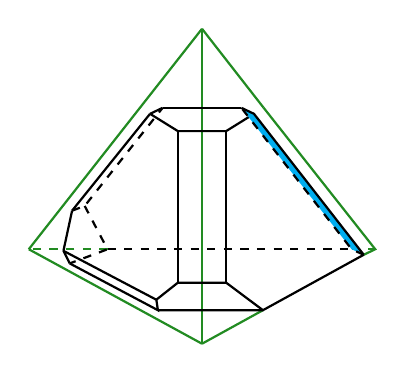
\begin{tikzpicture}[thick,scale=2]
\coordinate (A1) at (0,2);
\coordinate (A11) at (-0.39,1.5);
\coordinate (A111) at (-0.25,1.498);
\coordinate (A112) at (-0.33,1.46);
\coordinate (A12) at (0.39,1.5);
\coordinate (A121) at (0.25,1.498);
\coordinate (A122) at (0.33,1.46);
\coordinate (A13) at (0,1.25);
\coordinate (A131) at (-0.153,1.35); 
\coordinate (A132) at (0.153,1.35); 
\coordinate (A2) at (0,0); 
\coordinate (A21) at (-0.387,0.213); 
\coordinate (A211) at (-0.29,0.2795); 
\coordinate (A212) at (-0.28,0.213); 
\coordinate (A22) at (0.387,0.213); 
\coordinate (A23) at (0,0.5); 
\coordinate (A231) at (-0.153,0.388); 
\coordinate (A232) at (0.153,0.388); 
\coordinate (A3) at (-1.1,0.6);
\coordinate (A31) at (-0.9,0.49);
\coordinate (A311) at (-0.88,0.59);
\coordinate (A312) at (-0.84,0.51);
\coordinate (A32) at (-0.8,0.976);
\coordinate (A321) at (-0.825,0.845);
\coordinate (A322) at (-0.745,0.875);
\coordinate (A33) at (-0.6,0.6);
\coordinate (A4) at (1.1,0.6);
\coordinate (A41) at (1.027,0.565);
\coordinate (A42) at (0.95,0.6);
%\draw[draw=none,fill=cyan!40,opacity=0.5] (A42)--(A41)--(A121)--(A122)-- cycle;
\draw[draw=ForestGreen]  (A3)--(A2);
\draw[draw=ForestGreen]  (A1)--(A12);
\draw[draw=ForestGreen] (A2)--(A22);
\draw[draw=ForestGreen] (A2) -- (A1);
\draw[draw=ForestGreen] (A3)--(A1);
\draw[draw=ForestGreen,dashed]  (A33) -- (A3);
\draw[draw=ForestGreen,dashed]  (A42) -- (A4);
\draw[draw=ForestGreen] (A41)--(A4)--(A12);
 \draw[draw=black,fill=none]   (A321)--(A311);
 \draw[draw=black,fill=none] (A212)-- (A22) -- (A41);
\draw (A311)--(A312);
\draw (A111)--(A121);
\draw (A111)--(A112);
\draw (A311)--(A211)--(A212) --(A312);
\draw (A112)--(A321);
\draw[dashed] (A321)--(A322)--(A111);
\draw  (A211)--(A231)--(A232)--(A22);
\draw[dashed]  (A33) -- (A42);
\draw (A231) -- (A131) -- (A132) -- (A232) -- cycle;
\draw[dashed] (A322) -- (A33) -- (A312);
\draw (A112) -- (A131) --(A132)--(A122);
\fill[cyan] (A41) -- (A42) -- (A121)--(A122)--cycle;
\draw[dashed]  (A41) -- (A42) -- (A121); 
\draw (A41)--(A122) --(A121);
\end{tikzpicture}} \quad\quad  
\raisebox{1em}{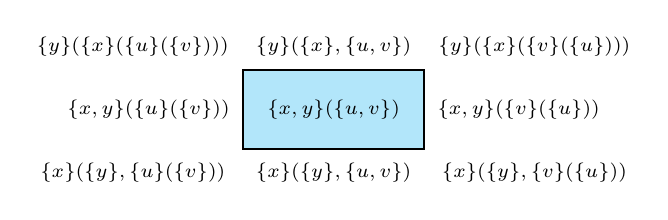
\begin{tikzpicture}[thick]
\coordinate (S1) at (-0.15,0);
\coordinate (S2) at (2.15,0);
\coordinate (S3) at (2.15,1);
\coordinate (S4) at (-0.15,1);
\draw[fill=cyan,opacity=0.3] (S1)--(S2)--(S3)--(S4)-- cycle;
\draw (S1)--(S2)--(S3)--(S4)-- cycle;
\node (s1) at (-1.55,-0.3) {\scriptsize $\{x\}(\{y\},\{u\}(\{v\}))$};
\node (s2) at (3.55,-0.3) {\scriptsize $\{x\}(\{y\},\{v\}(\{u\}))$};
\node (s4) at (-1.55,1.3) {\scriptsize $\{y\}(\{x\}(\{u\}(\{v\})))$};
\node (s3) at (3.55,1.3) {\scriptsize $\{y\}(\{x\}(\{v\}(\{u\})))$};
\node (s14) at (-1.35,0.5) {\scriptsize $\{x,y\}(\{u\}(\{v\}))$};
\node (s23) at (3.35,0.5) {\scriptsize $\{x,y\}(\{v\}(\{u\}))$};
\node (s12) at (1,-0.3) {\scriptsize $\{x\}(\{y\},\{u,v\})$};
\node (s34) at (1,1.3) {\scriptsize $\{y\}(\{x\},\{u,v\})$};
\node (s) at (1,0.5) {\scriptsize $\{x,y\}(\{u,v\})$};

\end{tikzpicture}}
\caption{A truncated simplex. \label{hemiassoc}}
\end{figure}

We recover associahedra and permutohedra as  linear and complete graphs, respectively: 

$$\begin{array}{ll}
\hyper{K}^X= \set{\set{x_1},\ldots,\set{x_n},\set{x_1,x_2},\ldots,\set{x_{n-1},x_n},\set{x_1,\ldots x_n}}, \\
\hyper{P}^X= \set{\set{x_1},\ldots,\set{x_n},\set{x_1,\ldots x_n}} \cup \setc{\set{x_i,x_j}}{1\leq i\neq j\leq n},
\end{array}$$




% !TEX root = ../Coherence.tex

\section{Topological coherence} 
\label{s:polycoherence}

%%%%%%%%%%%%%%%%%%%%%%%%%%%%%%%%%%

\subsection{Coherence \`a la Van Kampen}

Let $X$ be a regular CW complex, and let $X_k$, $k\geq 0$ denote its $k$-skeleton. 
\correction{
For an edge $e$ of $X$, denote its attaching map $f_e : \mathbb{S}^0 \to X_0$.
Consider the category $\mathcal{A}(X)$ with set of objects $X_0$, and generating morphisms $\alpha_e: f_e(-1) \to f_e(1)$ and $\alpha_e^{-1}: f_e(1) \to f_e(-1)$ for each edge $e \in X_1$.} 
A \defn{combinatorial path} on $X$ is a composable sequence of $\alpha$ and $\alpha^{-1}$ morphisms (a \emph{word} in $\alpha$ and $\alpha^{-1}$).
Two combinatorial paths \correction{$\gamma, \gamma' \in \mathcal{A}(X)(x,y)$} with the same endpoints are said to be \defn{parallel}.

\correction{
    Let $A$ be a $2$-cell of $X$.
    For any $x \in A_0$, the attaching map $f_A : \mathbb{S}^1 \to X_1$ of $A$ defines a morphism $\gamma_A \in \mathcal{A}(X)(x,x)$, given by the sequence of edges $e_1,\ldots,e_n$ in its image starting at~$x$ and respecting the anti-clockwise orientation of $\mathbb{S}^1$.
    Here, one selects $\alpha_{e_i}$ if the orientation of $f_A$ restricted to $e_i$ agrees with the one of $f_{e_i}$, and $\alpha_{e_i}^{-1}$ otherwise.}
Two parallel combinatorial paths $\gamma, \gamma'$ are said to be \defn{elementary combinatorially homotopic} if they differ exactly by a relation of the form $\gamma_A = \id_x$, for some $2$-cell $A$ \correction{and vertex $x$ of $A$}.
That is, one can rewrite $\gamma$ into $\gamma'$ or $\gamma'$ into $\gamma$ by replacing some (possibly empty) subword of $\gamma$ with an equivalent subword using a relation $\gamma_A = \id_x$.
More generally, two parallel combinatorial paths are \defn{combinatorially homotopic} if they are related by a sequence of elementary combinatorial homotopies.

\correction{
The quotient of the category $\mathcal{A}(X)$ by the relations $\alpha \alpha^{-1}=\alpha^{-1}\alpha=\id$ is the free groupoid $\mathcal{F}(X)$ generated by the $\alpha$ morphisms.
Let $\mathcal{C}(X)$ denote the further quotient of the groupoid $\mathcal{F}(X)$ by the relations $\gamma_A=\id_x$ for some choice of $x$, for each $2$-cell $A$ of $X$.
That is, the quotient of $\mathcal{F}(X)$ by the combinatorial homotopy equivalence relation.
Note that the definition of $\mathcal{C}(X)$ does not depend on the choice of $x$, for every $2$-cell $A$.
Indeed, if $x'\neq x \in A_0$ defines a relation $\gamma_A'=\id_{x'}$, we have $\gamma_A'=\delta \gamma_A \delta^{-1}$ in $\mathcal{F}(X)$, where $\delta$ is the oriented path between $x$ and $x'$. 
Thus, a path~$\gamma$ can be rewritten into $\gamma'$ using $\gamma_A=\id_x$ if and only if it can be rewritten using $\gamma_A'=\id_{x'}$.}

\correction{
Let $\Pi(X)$ denote the \defn{fundamental groupoid }of $X$, that is the groupoid with objects the points of $X$ and morphisms the homotopy classes of paths between them.}

\begin{thm}
\label{thm:top-coherence}
    Any two parallel combinatorial paths on $X$ are combinatorially homotopic if and only if every path component of $X$ is simply connected.
\end{thm}

\begin{proof}
    \correction{
    For $Y \subset X$, let us write $\Pi(X)Y$ for the full subcategory of the fundamental groupoid of $X$ spanned by $Y$.
    Then, we have an isomorphism of groupoids \[ \Pi(X)X_0 \cong \mathcal{C}(X) \ . \]}
    To show this, one proceeds in three steps. 
    First, one shows that the fundamental groupoid \correction{$\Pi(X_1)X_0$} of the $1$-skeleton of $X$ is free on the homotopy classes of maps generated by the attaching maps of the $1$-cells, that is, free on the $\alpha$-morphisms \cite[9.1.5]{Brown2006}.
    Thus, one gets \correction{$\Pi(X_1)X_0 \cong \mathcal{F}(X)$}. 
    Second, one shows that the fundamental groupoid $\Pi(X_2)X_0$ of the $2$-skeleton of $X$ is the free groupoid $\Pi(X_1)X_0$ modulo the relations $\gamma_A=1$, for $A$ a $2$-cell of $X$ \cite[9.1.6]{Brown2006}. 
    This is done through repeated application of the Seifert--Van Kampen theorem; one then has \correction{$\Pi(X_2)X_0 \cong \mathcal{C}(X)$}.
    Third, one shows that the inclusion of $X_2$ in $X$ induces an isomorphism of fundamental groupoids \correction{$\Pi(X_2)X_0 \cong \Pi(X)X_0$} \cite[9.1.7]{Brown2006}, which concludes the proof of the isomorphism \correction{$\Pi(X)X_0 \cong \mathcal{C}(X)$}.
    The theorem then follows, since every path component of $X$ is simply connected if and only if its fundamental groupoid $\Pi(X)$ is trivial, \correction{which holds if and only if its full subcategory $\Pi(X)X_0$ is trivial.}  
\end{proof}

\correction{
Let us say that $X$ is \defn{combinatorially connected} if there is a combinatorial path between any two vertices of $X$. 
In the course of the preceding proof, we have in particular showed the following.
\begin{corollary}
    \label{cor:combinatorially-connected}
    A regular CW complex $X$ is combinatorially connected if and only it is connected.
\end{corollary}
Note also that any CW complex is locally path connected, and therefore is connected if and only if it is path connected. %Hatcher Appendix A
}

%%%%%%%%%%%%%%%%%%%%%%%%%%%%%%%%%%

\subsection{Coherence \`a la Morse}

Let $X\subset \R^n$ be a polyhedral complex. 
Let $\vec v \in \R^n$ be \defn{generic} on the edges of $X$, meaning that for any pair of vertices $x,y \in X$ belonging to the same edge of $X$, we have $\langle \vec v , x \rangle \neq \langle \vec v, y\rangle$.  
Such a generic vector $\vec v$ induces a natural orientation on the edges of $X$, directed from the source vertex where the functional $\langle \vec v, - \rangle$ is minimal to the target vertex where it is maximal. 

In general, for any face $F \subset X$ of $X$, there is a unique \defn{source} vertex $\so(F)$ such that all its adjacent edges $e \subset F$ are outgoing, and a unique \defn{sink} vertex $\sk(F)$ whose adjacent edges are all incoming.
\correction{More generally, a vertex whose adjacent edges $e \subset X$ are all incoming is called a \defn{local sink}, and when $X$ has only one such vertex, we call it \defn{global sink} and denote it by $\sk(X)$.}

Let $H:=\{y \in \R^n \ | \ \langle \vec v , y \rangle = 0\}$ be the linear hyperplane orthogonal to $\vec v$.  
For every vertex $x \in X$, choose $\varepsilon >0$ such that the interval between $\langle \vec v , x \rangle$ and $\langle \vec v , x \rangle + \varepsilon$ does not contain the image of any other vertex under the ``height" function $\langle \vec v, - \rangle$. 

\begin{definition}
    The \defn{outgoing link} $\oLk(x,X)$ of a vertex $x \in X$ is the intersection $\mathcal{F} \cap (H+x+\varepsilon \vec v)$ of the family of faces $\mathcal{F}(x,X):=\{ F \subset X \ | \ \so(F)=x \}$ with the affine hyperplane $H+x+\varepsilon \vec v$. 
\end{definition}

\correction{
    Recall from \cite[Sec.~2.1]{Ziegler95} that the \defn{vertex figure} $P/x$ of a polytope $P$ at a vertex $x$ is obtained by cutting $P$ by a hyperplane that cuts off the single vertex $x$. 
    Such a cut establishes a bijection between the $(k-1)$-faces of $P/x$ and the $k$-faces of $P$ which contain $x$ \cite[Prop.~2.4]{Ziegler95}. 
\begin{lemma}
    \label{l:vertex-figure}
    For any $k\geq 0$, there is a bijection between the $k$-faces of $\mathcal{F}(x,X)$ and the $(k-1)$-faces of $\oLk(x,X)$.
\end{lemma}
\begin{proof}
    Each maximal face of $\mathcal{F}(x,X)$ with respect to inclusion is a polytope $P$, for which the intersection $P \cap (H+x+\varepsilon \vec v)$ is the vertex figure $P/x$ of $P$ at $x$. 
    By \cite[Prop.~2.4]{Ziegler95}, there is a bijection between the $k$-faces of $P$ and the $(k-1)$-faces of $P/x$.
    Collecting these bijections for all maximal faces of $\mathcal{F}(x,X)$, and making the appropriate identifications, we get the desired global bijection.
\end{proof}}

\correction{In this Section we shall focus on polyhedral complexes whose outgoing links are connected.}

\begin{proposition}
    \label{lemma:outgoing-link}
    Let $X$ be a polyhedral complex.
    If there is a generic vector $\vec v \in \R^n$ such that the outgoing link of every vertex is connected, then every path component of $X$ is simply connected.
\end{proposition}

\begin{proof}
    Let $\vec v \in \R^n$ be generic with respect to $X$, and suppose that the outgoing link of every vertex is connected. 
    Since $\vec v$ is generic on edges, it defines a Morse function $\langle \vec v , -\rangle$ on $X$, in the sense of \cite[Def.~2.2]{bestvinaMorseTheoryFiniteness1997}.
    As in classical Morse theory, one can determine the homotopy type of $X$ by considering its successive level sets. 
    For $t \in \R$ denote by $X_t$ the closed subspace of $X$ containing points $x$ such that $\langle x, \vec v \rangle$ is at least $t$.
    Let $x$ be a vertex of $X$ of height $h=\langle x, \vec v \rangle$.
    Observe first that $X_{h+\epsilon}$, for some small $\epsilon>0$, is homotopy equivalent to $X_{h'}$ where $h' > h$ is the next greater height at which there is a vertex.
    That is, the homotopy type of $X$ can only change at vertices  \cite[Lem.~2.3]{bestvinaMorseTheoryFiniteness1997}.
    Then, one proves that $X_h$ is homotopy equivalent to the pushout of $X_{h+\epsilon}$ with the cone over the outgoing link of $x$ along the outgoing link of $x$  \cite[Lem.~2.5]{bestvinaMorseTheoryFiniteness1997}.
    By our assumption, the outgoing link of $x$ is connected, and thus the cone over it is simply connected. 
    Since the pushout of simply connected spaces over a connected space is always simply connected (this is an application of the Seifert--Van Kampen theorem), we obtain by induction that every path component of $X$ is simply connected \cite[Point (3) of Cor.~2.6]{bestvinaMorseTheoryFiniteness1997}.
\end{proof}

The converse of \cref{lemma:outgoing-link} is not true in general: many simply connected polyhedral complexes, as the one represented in \cref{fig:outgoingpoly}, have disconnected outgoing links, for many (sometimes for all) choices of generic orientation vectors. 

\begin{figure}[h!]
\centering
\resizebox{0.4\linewidth}{!}{
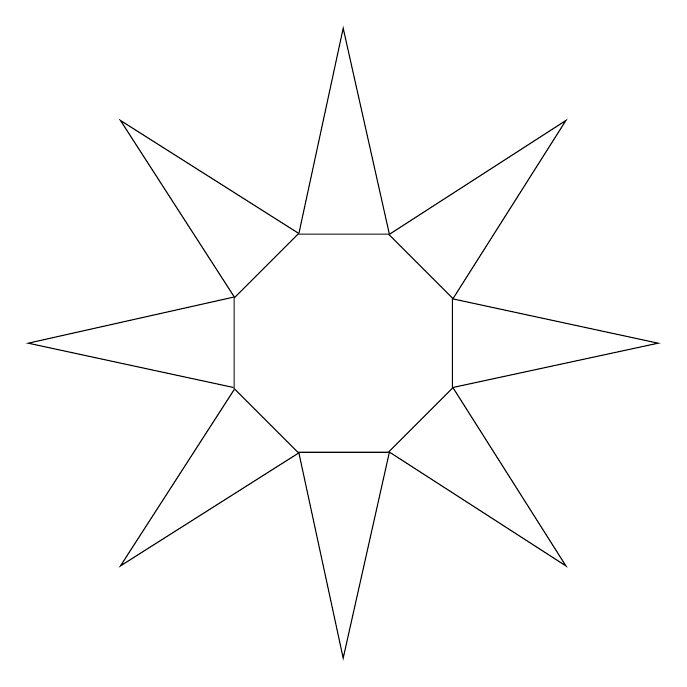
\begin{tikzpicture}
    \node[regular polygon,
    draw,
    regular polygon sides = 8, minimum size = 3cm] (p) at (0,0) {};
    \draw[-] (p.202.5)--(180:4)--(p.157.5);
    \draw[-] (p.157.5)--(135:4)--(p.112.5);
    \draw[-] (p.112.5)--(90:4)--(p.67.5);
    \draw[-] (p.67.5)--(45:4)--(p.22.5);
    \draw[-] (p.22.5)--(0:4)--(p.-22.5);
    \draw[-] (p.-22.5)--(-45:4)--(p.-67.5);
    \draw[-] (p.-67.5)--(-90:4)--(p.-112.5);
    \draw[-] (p.-112.5)--(-135:4)--(p.-157.5);
\end{tikzpicture}}
\caption{A simply connected polyhedral complex which admits disconnected outgoing links for every choice of generic vector.}
\label{fig:outgoingpoly}
\end{figure}

\correction{An important class of complexes which have connected outgoing links are polytopes, which will be our main object of study in the next sections.}

\begin{proposition}
\label{prop:polytopes}
    Let $P \subset \R^n$ be a polytope, and let $\vec v \in \R^n$ be generic with respect to $P$. 
    Then, the outgoing link of every vertex of $P$ is connected.
\end{proposition}

\begin{proof}
    Define the linear hyperplane $H:=\{y \in \R^n \ | \ \langle \vec v, y \rangle = 0\}$, and consider the two half-spaces $H^{-}:=\{y \in \R^n \ | \ \langle \vec v, y \rangle < 0\}$ and $H^{+}:=\{y \in \R^n \ | \ \langle \vec v, y \rangle < 0\}$.
    Since $\vec v$ is not perpendicular to any edge of $P$, it defines a partition of the vertices of the vertex figure $P/x$ into two connected components: the vertices that lie in $H^{-}$, which correspond to incoming edges of $P$ at $x$, and the vertices that lie in $H^{+}$, which correspond to outgoing edges of $P$ at $x$.
    Thus, the outgoing link of $x$ is connected, and the proof is complete.
\end{proof}

\correction{From now on we shall suppose that the polyhedral complexes $X$ that we consider are endowed with a regular CW structure and provided with a generic vector $\vec v$.
Combining \cref{lemma:outgoing-link} with \cref{thm:top-coherence}, we have that any polyhedral complex $X$ whose outgoing links are connected satisfies the property that ``any two parallel combinatorial paths on $X$ are combinatorially homotopic''.
We shall now derive this same result by following an alternative, more combinatorial path (indeed!), getting close to the proof of \cite[Thm~3.1]{MacLane63}.}

A combinatorial path $\gamma$ on $X$ is \defn{oriented} if for any pair $(e, f)$ of consective edges in~$\gamma$, we have that $\sk(e)=\so(f)$.  
When no ambiguity arises, we will omit the adjective ``combinatorial" and say only ``oriented path".

\correction{Let us start with a small Lemma.
In the rest of this Section we shall use the notion of combinatorial connectedness, which as we have seen in \cref{cor:combinatorially-connected}, is equivalent to connectedness for the spaces we consider.
\begin{lemma}
    \label{l:unique-sink}
    Let $X$ be a polyhedral complex with generic vector $\vec v$ such that the outgoing link of every vertex is combinatorially connected. 
    Let $e,e'$ be two edges of $X$ such that $\so(e)=\so(e')$, and suppose that there are oriented paths from $\sk(e)$ and $\sk(e')$ to local sinks~$s$ and~$s'$, respectively. 
    Then, we have $s=s'$.
\end{lemma}
\begin{proof}
    Define the \emph{height} $\frakh(x)$ of a vertex $x$ as the length of the longest oriented path in $X$ starting at $x$.
    Since $\vec v$ is generic and $X_0$ is finite, this is well-defined.
    We proceed by induction on $\frakh(x)$.
    The statement holds vacuously for vertices $x$ such that $\frakh(x)=0$.
    Suppose that the assertion above holds for all vertices $x \in X$ such that $\frakh(x)=n$, and consider an $x$ with $\frakh(x)=n+1$.
    Since the outgoing link $\oLk(x,X)$ is combinatorially connected, there is a combinatorial path $\theta$ in $\oLk(x,X)$ between the vertices corresponding to $e$ and $e'$ (\cref{l:vertex-figure}).
    $\theta$ determines a sequence of edges $e_0 \eqdef e, e_1, \ldots, e_k, e' \defeq e_{k+1}$ of $X$ with $\so(e_i)=x$ for all $0 \leq i \leq k+1$.
    Moreover, each consecutive pair $e_i,e_{i+1}$ determines a $2$-face~$F_{i+1}$ of $X$.
    Now, choose for each $e_i$ with $1 \leq i \leq k$, an oriented path of maximal length starting at $\sk(e_i)$ and passing through $\sk(F_{i})$.
    Each of these paths ends at a local sink $s_i$, including $s_0 \eqdef s$ and $s_{k+1} \eqdef s'$. 
    Since we have $\frakh(\sk(e_i))<\frakh(x)$ for all $0 \leq i \leq k+1$, we can apply induction to the two oriented paths from $\sk(e_i)$ to $s_i$ and $s_{i+1}$, which gives~$s_i=s_{i+1}$.
    Therefore, we have $s=s_0=s_1=\cdots =s_k=s_{k+1}=s'$, as desired.
\end{proof}}

Two parallel oriented paths are said to be \defn{elementary combinatorially homotopic} if they are as non-oriented paths. 
They are \defn{combinatorially homotopic} if they are related by a sequence of elementary combinatorial homotopies between oriented paths. 

The following \cref{l:oriented} and its consequence \cref{p:second-proof} expresses in topological terms the original proof technique used by Mac Lane in \cite[Thm~3.1]{MacLane63}.
\correction{Note that this \cref{l:oriented} involves first \emph{oriented} paths, while \cref{p:second-proof} treats the general, non-oriented case.}

\begin{proposition}
\label{l:oriented}
    Let $X$ be a polyhedral complex, and let $\vec v$ be generic on the edges of $X$. 
    \correction{Consider the following three properties:
    \begin{enumerate}
        \item[(i)] the outgoing link of every vertex is combinatorially connected,
        \item[(ii)] there is a unique global sink in every connected component,
        \item[(iii)] any two parallel \emph{oriented} combinatorial paths on $X$ are combinatorially homotopic.
    \end{enumerate}
    Then, $X$ satisfies (i) if and only if it satisfies (ii) and (iii).}
\end{proposition}

\begin{proof}
    \correction{First, we prove that (i) implies (ii). 
    Suppose that there are two local sinks~$s_1$ and~$s_2$ in the same connected component of $X$.
    Consider a combinatorial path $\gamma$ between~$s_1$ and~$s_2$, whose existence is garanteed by \cref{cor:combinatorially-connected}.
    We proceed by induction on the number of \emph{peaks} in $\gamma$, that is the number of vertices $x$ which are the source $\so(e)=x=\so(e')$ of two edges $e,e'$ of $\gamma$.
    The path $\gamma$ has at least a peak, otherwise $s_1$ and $s_2$ would not be both local sinks. 
    If $\gamma$ has a unique peak, \cref{l:unique-sink} implies that $s_1=s_2$.
    Now suppose that for any $k \leq n$, if $\gamma$ has $k$ peaks, then we have $s_1=s_2$. 
    If $\gamma$ has $n+1$ peaks, consider the first peak $x=\so(e)=\so(e')$ of $\gamma$. 
    By \cref{l:unique-sink}, there is an oriented path $\delta$ from $\sk(e')$ to $s_1$. 
    Replacing the initial section of $\gamma$ ending in $e’$ by $\delta$, we get a path with $n$ peaks, and by the induction hypothesis we get $s_1=s_2$, completing the proof.}

    \correction{Second, we prove that (i) implies (iii).
    Let us assume that $X$ is connected, otherwise we apply the same reasoning to each connected component. 
    From the preceding paragraph, we know that $X$ has a unique sink $\sk(X)$.}
    Suppose that the outgoing link of every vertex is \correction{combinatorially} connected. 
    Let $\gamma$ and $\gamma'$ be two parallel oriented paths between two vertices $x$ and $y$. 
    We prove that they are combinatorially homotopic. 
    We proceed by induction on the maximal length $m$ of an oriented path between $x$ and $y$ in $X$. 
    Without loss of generality, we can suppose that $y=\sk(X)$, since if $y\neq\sk(X)$ we can always find an oriented path between $y$ and $\sk(X)$.
    The cases when $m=0$ and $m=1$ are trivial. 
    Suppose that the hypothesis holds up to $m=k-1, k\geq 2$, and consider two paths $\gamma$ and $\gamma'$ for which $m=k$. 
    Let $e$ and $e'$ denote the edges of $\gamma$ and $\gamma'$ that are adjacent to $x$. 
    We examine three cases.
    \begin{enumerate}
        \item If $e=e'$, we can apply the induction hypothesis to $\gamma \setminus e$ and $\gamma' \setminus e'$. 
        \item If $e \neq e'$ and both edges are on the same $2$-face $F$ of $X$, then using the induction hypothesis we have that $\gamma$ and $\gamma'$ are respectively combinatorially homotopic to the paths $\delta$ and $\delta'$ defined as follows: they go from $x=\so(F)$ to $\sk(F)$ by the unique path containing $e$ and $e'$, respectively, and then from $\sk(F)$ to $y$ along the same arbitrary oriented path. 
        Since $\delta$ and $\delta'$ are combinatorially homotopic by definition, the conclusion follows from the transitivity of the combinatorial homotopy equivalence relation. 
        \item Suppose that $e\neq e'$, and that $e$ and $e'$ are \emph{not} on the same $2$-face of $X$. 
        Since the outgoing link of $x$ is \correction{combinatorially} connected, there exists a \correction{combinatorial} path $\theta$ between \correction{the vertices corresponding to} $e$ and $e'$ in this link \correction{(\cref{l:vertex-figure})}. 
        For every edge $e_i$ of $X$ in the path $\theta$, choose an oriented path $\gamma_i$ in $X$ from $x$ to $y=\sk(X)$ going through $e_i$. 
        Now apply Point (2) above to every pair of parallel oriented paths $(\gamma_i, \gamma_{i+1})$ with $e_i$ and $e_{i+1}$ consecutive in $\theta$, and conclude again by transitivity of the combinatorial homotopy equivalence relation. 
    \end{enumerate}

    \correction{Finally, we prove that (ii) and (iii) imply (i).}
    Suppose that every pair of parallel oriented combinatorial paths are combinatorially homotopic. 
    We show that for any vertex $x$, its outgoing link is \correction{combinatorially} connected. 
    Indeed, take two edges $e,e'$ of $X$ with source $x$, and consider their extensions to oriented paths $\gamma, \gamma'$ from $x$ to $\sk(X)$. 
    By hypothesis, these two paths are combinatorially homotopic, that is, there is a sequence of parallel oriented paths from $\gamma$ to $\gamma'$. 
    The collection of first edges in each of these paths defines a \correction{combinatorial} path between $e$ and $e'$ in the outgoing link of $x$. 
    Thus, this link is \correction{combinatorially} connected. 
\end{proof}

\begin{rem}
    Note that the existence and uniqueness of a global sink is one of the basic, very useful facts about polytopes, see \cite[Thm.~3.7]{Ziegler95}.
\end{rem}

\begin{thm}
\label{p:second-proof}
    Let $X$ be a polyhedral complex with generic vector $\vec v$ \correction{such that the outgoing link of every vertex is combinatorially connected.}
    Then, any two parallel combinatorial paths on $X$ are combinatorially homotopic.
\end{thm}

\begin{proof} 
    \correction{Assume that $X$ is connected, otherwise apply the argument to each connected component.
    By \cref{l:oriented}, the polyhedral complex $X$ admits a unique global sink $\sk(X)$ and} the conclusion holds for \emph{oriented} paths.  
    Let us show that this implies the non-oriented version.
    Let $\gamma$ be a non-oriented combinatorial path on $X$ between $x$ and $y$.
    For every vertex $z$ along $\gamma$, one can choose an oriented path $\delta_z$ from $z$ to $\sk(X)$. 
    We observe that for any edge $e: z \to z'$ of $\gamma$, the oriented paths $\delta_z$ and $\delta_{z'}e$ are combinatorially homotopic by hypothesis. 
    Going from $x$ to $y$ inductively one edge at a time and using transitivity of the homotopy equivalence relation, one obtains that $\gamma$ is combinatorially homotopic to $\delta_y^{-1}\delta_x$. 
    Taking another combinatorial path $\gamma'$ parallel to $\gamma$, the same argument shows that $\gamma'$ is combinatorial homotopic to $\delta_y^{-1}\delta_x$.
    Thus $\gamma$ and $\gamma'$ are combinatorially homotopic, which completes the proof. 
\end{proof}

As \cref{lemma:outgoing-link} shows, the class of polyhedral complexes to which \cref{p:second-proof} applies is a strict subclass of simply connected complexes.
This implies that the converse of \cref{p:second-proof} does not hold, and thus that Mac Lane's original proof is far from reaching the full generality of \cref{thm:top-coherence}.
However, it will be sufficient for our purposes, since --as we have seen in \cref{prop:polytopes}-- it applies to any polytope.
\correction{Another feature of generically oriented polyhedral complexes is that their $1$-skeleton defines abstract rewriting systems which are terminating and confluent, as we now show.}

%%%%%%%%%%%%%%%%%%%%%%%%%%%%%%%%%%

\subsection{Rewriting systems}
\label{ss:abstract-rewriting}

\correction{
    We refer to \cite{baaderTermRewritingAll1998} for more details on rewriting systems. 
\begin{definition}
    An \defn{abstract rewriting system} is a set $A$ together with a binary relation~$\to$. 
\end{definition}
We denote by $\xrightarrow{*}$ the reflexive and transitive closure of ${\to}$. 
We say that $(A,\to)$ is \defn{locally confluent} (resp.\ \defn{confluent}) if for all $a,a_1,a_2 \in A$ such that $a_1 \leftarrow a \to a_2$ (resp.\ $a_1 \xleftarrow{*} a \xrightarrow{*} a_2$), there exists a term $b$ with $a_1 \xrightarrow{*} b \xleftarrow{*} a_2$.  
The diagram}
\begin{center}
  \begin{tikzcd}
    & a \arrow[ld] \arrow[rd] &                     \\
a_1 \arrow[rd, "*"'] &                         & a_2 \arrow[ld, "*"] \\
    & b                       &                    
\end{tikzcd}
\end{center}
\correction{is called a \defn{local confluence diagram}.
A rewriting system is \defn{terminating} if every reduction sequence $a \to a_1 \to a_2 \to \cdots$ eventually must terminate.
An element $a \in A$ is \defn{reducible} if there exists an $a' \in A$ such that $a \to a'$; otherwise it is called \defn{irreducible}.
We say that $b$ is a \defn{normal form} of $a$ if $a \xrightarrow{*} b$ and $b$ is irreducible.}

\correction{
    Given a polyhedral complex $X$ and a generic vector $\vec v$, one can consider the abstract rewriting system defined by $\vec v$ on the vertices of $X$.
\begin{definition}
    The \defn{vertices rewriting system} is the pair $(X_0,\to)$ made of the set of vertices $X_0$ of $X$, together with the following relation: we have $x \to y$ if $x$ and $y$ are vertices of the same edge and $\langle v, x \rangle < \langle v, y \rangle$.
\end{definition}
According to this definition, we have $x \xrightarrow{*} y$ if and only if there is an oriented path from $x$ to $y$ in~$X_1$. 
The hypothesis of \cref{p:second-proof} imposes that the rewriting system $(X_0,\to)$ is terminating and confluent.
\begin{proposition}
    Let $X$ be a polyhedral complex and $\vec v$ be a generic vector. 
    If the outgoing link of every vertex is combinatorially connected, the rewriting system $(X_0,\to)$ is terminating and confluent. 
\end{proposition}
\begin{proof}
    Since $\vec v$ is generic, and thus strictly increasing along edges, it defines a partial order, and since the set $X_0$ is finite, the rewriting system $(X_0,\to)$ is terminating.
    By \cref{l:oriented}, there is a unique sink in each connected component of $X$.
    Confluence then follows: given any pair of vertices $x,y$ in the same connected component, since $\vec v$ is generic there are oriented paths $x \xrightarrow{*} s \xleftarrow{*} y$ to the global sink $s$ of this connected component. 
\end{proof}
\begin{corollary}
    The abstract rewriting system on the vertices of any oriented polytope~$P$ is terminating and confluent.
    Moreover, every pair of vertices admits a unique normal form~$\sk(P)$.
\end{corollary}
Recall that a polytope $P$ is \emph{simple} if each vertex of $P$ is incident to precisely $\dim P$ edges.
\begin{lemma}
    If a polytope $P$ is simple, then there is a bijection between the local confluence diagrams of $(P_0,\to)$ and the oriented boundaries of the $2$-faces of~$P$.
\end{lemma}
\begin{proof}
    When $P$ is simple, the vertex figure $P/x$ of every vertex $x$ is a simplex \cite[Prop.~2.16]{Ziegler95}, with each edge in $P/x$ corresponding to a $2$-face of $P$ (\cref{l:vertex-figure}). 
    Thus every pair of edges $e,e'$ with source $x=\so(e)=\so(e')$ determines a $2$-face of~$P$. 
\end{proof}
Not much more can be said at this level of generality. 
For the specific families of polytopes that we will consider in the next Section, the rewriting systems possess more structure (they are \emph{term} rewriting system) and deserve their own study, see \cite{CLA24} for more details.}

%Terminating and confluent
%Rewriting rules
%Critical pairs
% !TEX root = ../Coherence.tex

\section{Categorical coherence} 
\label{s:catoperads}
 
\subsection{Basic definitions}

Throughout this section we consider structures without units.
Unless otherwise stated, the adjective ``non-unital" will be implicitly assumed. 

\begin{definition} 
\label{def:catoperad}
A \defn{categorified non-symmetric operad} $\mathcal{P}$ is a collection $\left\{  \mathcal{P}(n)  \right\}_{n\in \mathbb{N}}$ of small categories equipped with bifunctors  
$$ \begin{array}{clll}
\circ_i&\colon& \mathcal{P}(n) \times
                    \mathcal{P}(k)
                    \longrightarrow \mathcal{P}(n+k-1) \ ,
                    & \text{for}\ 1 \leq i \leq n \ ,
\end{array}  $$
and for each $\kappa \in \mathcal{P}(m)$,  $\mu \in \mathcal{P}(n)$, $\nu \in \mathcal{P}(k)$, $1 \leq i \leq m$, $1 \leq j \leq n$ natural isomorphisms 
$$ \begin{array}{clll}
    \beta_{\kappa,\mu,\nu}&\colon& 
    (\kappa \circ_i \mu) \circ_{j+i-1} \nu  \overset{\cong}{\longrightarrow} \kappa \circ_i (\mu \circ_j \nu) \ , &  \\
    \theta_{\kappa,\nu,\mu}&\colon& 
    (\kappa \circ_i \nu) \circ_{j+k-1} \mu 
    \overset{\cong}{\longrightarrow} (\kappa \circ_j \mu) \circ_i \nu \ , & \text{when}\ i < j \ , 
\end{array}  $$
such that the following diagrams commute: the pentagonal \\
\begin{center}
\resizebox{\linewidth}{!}{
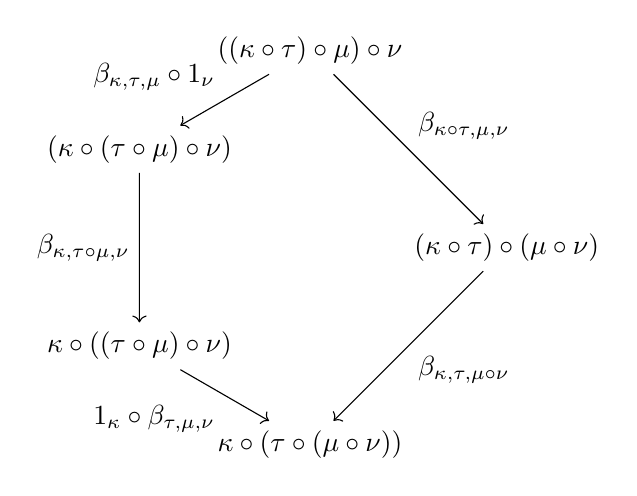
\begin{tikzpicture}[scale=2.5]
    \node (P1) at (0,1) {$((\kappa\circ\tau)\circ\mu)\circ\nu$};
    \node (P2) at (-0.866,0.5) {$(\kappa\circ(\tau\circ\mu)\circ\nu)$};
    \node (P3) at (-0.866,-0.5) {$\kappa\circ((\tau\circ\mu)\circ\nu)$};
    \node (P4) at (0,-1) {$\kappa\circ(\tau\circ(\mu\circ\nu))$};
    \node (P5) at (1,0) {$(\kappa\circ\tau)\circ(\mu\circ\nu)$} ;
    \draw[->] (P1)--(P2) node[midway,above left] {$\beta_{\kappa,\tau,\mu}\circ 1_\nu$};
    \draw[->] (P2)--(P3) node[midway,left] {$\beta_{\kappa,\tau\circ\mu,\nu}$};
    \draw[->] (P3)--(P4) node[midway,below left] {$1_\kappa \circ \beta_{\tau,\mu,\nu}$};
    \draw[->] (P1)--(P5) node[midway,above right] {$\beta_{\kappa\circ\tau,\mu,\nu}$};
    \draw[->] (P5)--(P4) node[midway,below right] {$\beta_{\kappa,\tau,\mu\circ\nu}$};
\end{tikzpicture} \quad 
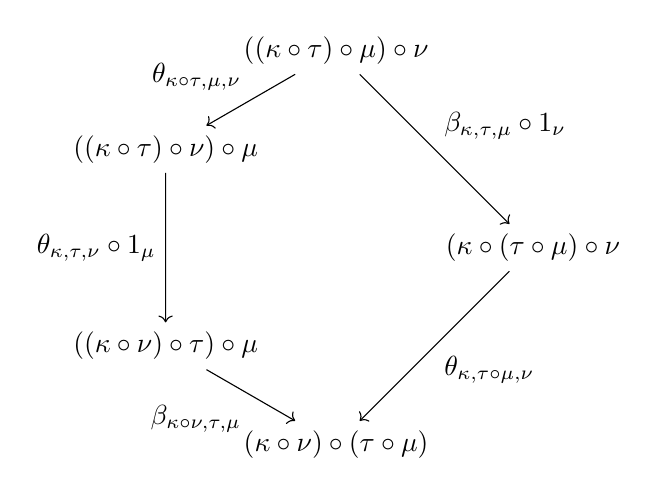
\begin{tikzpicture}[scale=2.5]
    \node (P1) at (0,1) {$((\kappa\circ\tau)\circ\mu)\circ\nu$};
    \node (P2) at (-0.866,0.5) {$((\kappa\circ\tau)\circ\nu)\circ\mu$};
    \node (P3) at (-0.866,-0.5) {$((\kappa\circ\nu)\circ\tau)\circ\mu$};
    \node (P4) at (0,-1) {$(\kappa\circ\nu)\circ(\tau\circ\mu)$};
    \node (P5) at (1,0) {$(\kappa\circ(\tau\circ\mu)\circ\nu$} ;
    \draw[->] (P1)--(P2) node[midway,above left] {$\theta_{\kappa\circ\tau,\mu,\nu}$};
    \draw[->] (P2)--(P3) node[midway,left] {$\theta_{\kappa,\tau,\nu}\circ 1_\mu$};
    \draw[->] (P3)--(P4) node[midway,below left] {$\beta_{\kappa\circ\nu,\tau,\mu}$};
    \draw[->] (P1)--(P5) node[midway,above right] {$\beta_{\kappa,\tau,\mu}\circ 1_\nu$};
    \draw[->] (P5)--(P4) node[midway,below right] {$\theta_{\kappa,\tau\circ\mu,\nu}$};
\end{tikzpicture} } \\
\end{center}

\begin{center}
\resizebox{0.5\linewidth}{!}{
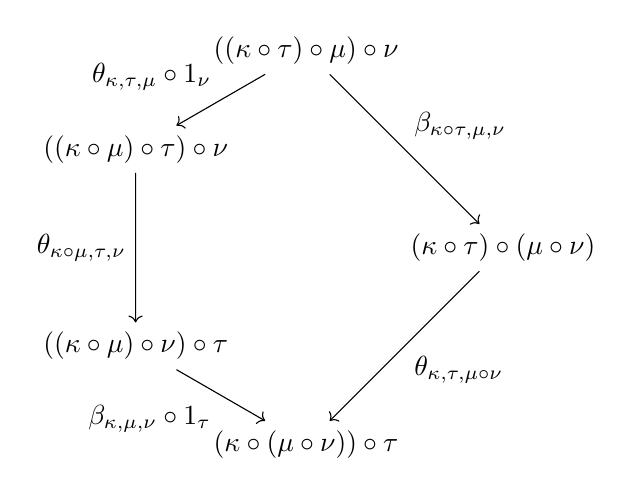
\begin{tikzpicture}[scale=2.5]
    \node (P1) at (0,1) {$((\kappa\circ\tau)\circ\mu)\circ\nu$};
    \node (P2) at (-0.866,0.5) {$((\kappa\circ\mu)\circ\tau)\circ\nu$};
    \node (P3) at (-0.866,-0.5) {$((\kappa\circ\mu)\circ\nu)\circ\tau$};
    \node (P4) at (0,-1) {$(\kappa\circ(\mu\circ\nu))\circ\tau$};
    \node (P5) at (1,0) {$(\kappa\circ\tau)\circ(\mu\circ\nu)$} ;
    \draw[->] (P1)--(P2) node[midway,above left] {$\theta_{\kappa,\tau,\mu}\circ 1_\nu$};
    \draw[->] (P2)--(P3) node[midway,left] {$\theta_{\kappa\circ\mu,\tau,\nu}$};
    \draw[->] (P3)--(P4) node[midway,below left] {$\beta_{\kappa,\mu,\nu}\circ 1_\tau$};
    \draw[->] (P1)--(P5) node[midway,above right] {$\beta_{\kappa\circ\tau,\mu,\nu}$};
    \draw[->] (P5)--(P4) node[midway,below right] {$\theta_{\kappa,\tau,\mu\circ\nu}$};
\end{tikzpicture}}
\end{center}

and hexagonal identities \\
\begin{center}
\resizebox{\linewidth}{!}{
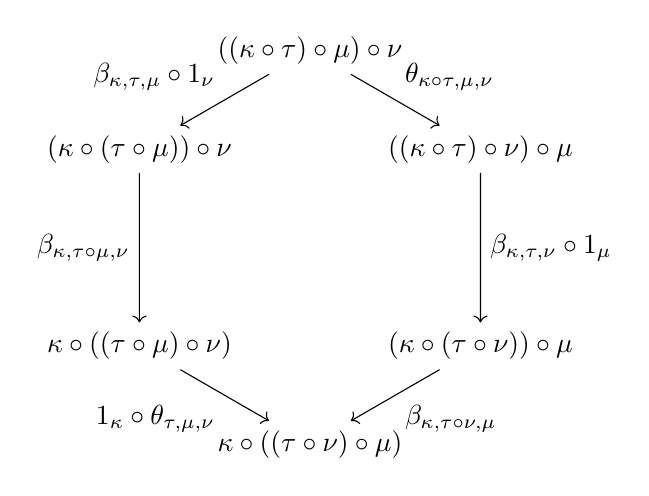
\begin{tikzpicture}[scale=2.5]
    \node (P1) at (0,1) {$((\kappa\circ\tau)\circ\mu)\circ\nu$};
    \node (P2) at (-0.866,0.5) {$(\kappa\circ(\tau\circ\mu))\circ\nu$};
    \node (P3) at (-0.866,-0.5) {$\kappa\circ((\tau\circ\mu)\circ\nu)$};
    \node (P4) at (0,-1) {$\kappa\circ((\tau\circ\nu)\circ\mu)$};
    \node (P5) at (0.866,0.5) {$((\kappa\circ\tau)\circ\nu)\circ\mu$} ;
    \node (P6) at (0.866,-0.5) {$(\kappa\circ(\tau\circ\nu))\circ\mu$};
    \draw[->] (P1)--(P2) node[midway,above left] {$\beta_{\kappa,\tau,\mu}\circ 1_\nu$};
    \draw[->] (P2)--(P3) node[midway,left] {$\beta_{\kappa,\tau\circ\mu,\nu}$};
    \draw[->] (P3)--(P4) node[midway,below left] {$1_\kappa \circ \theta_{\tau,\mu,\nu}$};
    \draw[->] (P1)--(P5) node[midway,above right] {$\theta_{\kappa\circ\tau,\mu,\nu}$};
    \draw[->] (P5)--(P6) node[midway,right] {$\beta_{\kappa,\tau,\nu}\circ 1_\mu$};
    \draw[->] (P6)--(P4) node[midway,below right] {$\beta_{\kappa,\tau\circ\nu,\mu}$};
\end{tikzpicture} \quad \quad
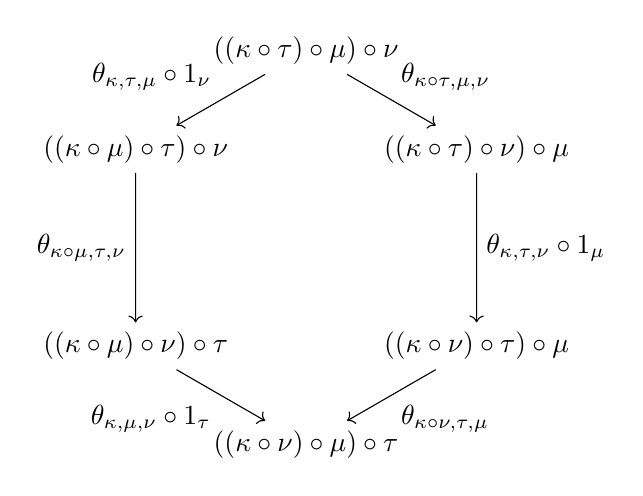
\begin{tikzpicture}[scale=2.5]
    \node (P1) at (0,1) {$((\kappa\circ\tau)\circ\mu)\circ\nu$};
    \node (P2) at (-0.866,0.5) {$((\kappa\circ\mu)\circ\tau)\circ\nu$};
    \node (P3) at (-0.866,-0.5) {$((\kappa\circ\mu)\circ\nu)\circ\tau$};
    \node (P4) at (0,-1) {$((\kappa\circ\nu)\circ\mu)\circ\tau$};
    \node (P5) at (0.866,0.5) {$((\kappa\circ\tau)\circ\nu)\circ\mu$} ;
    \node (P6) at (0.866,-0.5) {$((\kappa\circ\nu)\circ\tau)\circ\mu$};
    \draw[->] (P1)--(P2) node[midway,above left] {$\theta_{\kappa,\tau,\mu}\circ 1_\nu$};
    \draw[->] (P2)--(P3) node[midway,left] {$\theta_{\kappa\circ\mu,\tau,\nu}$};
    \draw[->] (P3)--(P4) node[midway,below left] {$\theta_{\kappa,\mu,\nu}\circ 1_\tau$};
    \draw[->] (P1)--(P5) node[midway,above right] {$\theta_{\kappa\circ\tau,\mu,\nu}$};
    \draw[->] (P5)--(P6) node[midway,right] {$\theta_{\kappa,\tau,\nu}\circ 1_\mu$};
    \draw[->] (P6)--(P4) node[midway,below right] {$\theta_{\kappa\circ\nu,\tau,\mu}$};
\end{tikzpicture}  } \quad \ .
\end{center}
\end{definition}
The diagrams above hold for all instances of composable $\beta$ and $\theta$; these depend on the indices $i,j,k$, which are omitted for the sake of readability. 
Observe that a categorified non-symmetric operad concentrated in arity $1$ is a non-symmetric monoidal category.

One can picture an object $\mu \in \mathcal{P}(n)$ as a planar tree with one vertex decorated by $\mu$, $n$ leaves and one root (a \defn{corolla}). 
The $\circ_i$ bifunctors then correspond to the operation of \defn{grafting} a corolla on top of another.
Iterated applications of the $\circ_i$ can be visualized as fully nested planar trees \cite[Def.~2.2]{laplante-anfossiDiagonalOperahedra2022a}, with vertices decorated by objects of $\mathcal{P}$, see \cref{fig:treeandnesting}. 

\begin{figure}[h!]
\centering
\resizebox{0.4\linewidth}{!}{
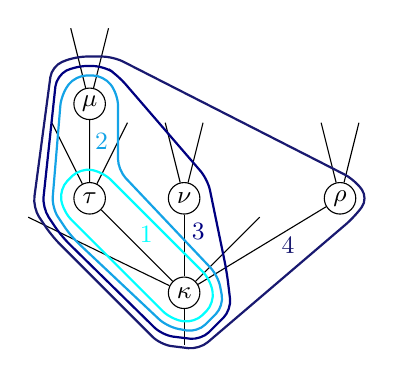
\begin{tikzpicture}[scale=1.2]
        \node (E)[circle,draw=black,minimum size=4mm,inner sep=0.1mm] at (-0,0) {\small $\kappa$};
        \node (F) [circle,draw=black,minimum size=4mm,inner sep=0.1mm] at (-1,1) {\small $\tau$};
        \node (A) [circle,draw=black,minimum size=4mm,inner sep=0.1mm] at (-1,2) {\small $\mu$};
        \node (q) [circle,draw=black,minimum size=4mm,inner sep=0.1mm] at (0,1) {\small $\nu$};
        \node (r) [circle,draw=black,minimum size=4mm,inner sep=0.1mm] at (1.65,1) {\small $\rho$};
        \node (x) [circle,draw=none,minimum size=4mm,inner sep=0.1mm] at (-0.4,0.62) {\color{Cyan} \small $1$};
        \node (y) [circle,draw=none,minimum size=4mm,inner sep=0.1mm] at (-0.875,1.6) {\color{Cerulean} \small $2$};
        \node (u) [circle,draw=none,minimum size=4mm,inner sep=0.1mm] at (0.15,0.65) {\color{NavyBlue} \small $3$};
        \node (v) [circle,draw=none,minimum size=4mm,inner sep=0.1mm] at (1.1,0.5) {\color{MidnightBlue} \small $4$};
        \draw[-] (0.8,0.8) -- (E)--(-1.65,0.8); 
        \draw[-] (-1.2,2.8) -- (A)--(-0.8,2.8); 
        \draw[-] (-0.2,1.8) -- (q)--(0.2,1.8);   
        \draw[-] (1.85,1.8) -- (r)--(1.45,1.8); 
        \draw[-] (E)--(0,-0.55); 
        \draw[-] (-1.4,1.8) -- (F)--(-0.6,1.8);   
        \draw[-] (E)--(F) node {};
        \draw[-] (E)--(q) node  {};
        \draw[-] (E)--(r) node {};
        \draw[-] (F)--(A) node {};
        \draw [Cyan,rounded corners,thick] (0.11,-0.32) -- (-0.14,-0.28) -- (-1.28,0.86) -- (-1.32,1.1) --  (-1.1,1.32) -- (-0.86,1.28) -- (0.28,0.14) -- (0.32,-0.11) -- cycle;
        \draw [Cerulean,rounded corners,thick] (0.14,-0.42) -- (-0.18,-0.36) -- (-1.2,0.6) -- (-1.4,0.9) -- (-1.3,2.1) -- (-1.15,2.3) -- (-0.85,2.3) -- (-0.7,2.1) --  (-0.7,1.3) -- (0.36,0.18) -- (0.42,-0.14) -- cycle;
        \draw [NavyBlue,rounded corners,thick] (0.18,-0.5) -- (-0.23,-0.45) -- (-1.3,0.6) -- (-1.5,0.9) --  (-1.35,2.3) --  (-1.15,2.4) --  (-0.85,2.4) --  (-0.7,2.3) --  (.25,1.2) -- (0.45,0.23) -- (0.5,-0.18) -- cycle;
        \draw [MidnightBlue,rounded corners,thick] (0.16,-0.6) -- (-0.25,-0.55) -- (-1.4,0.6) -- (-1.6,0.9) --  (-1.4,2.4) --  (-1.15,2.5) --  (-0.75,2.5) --  (1.8,1.2) --  (1.95,1) --  (1.8,0.8) -- cycle;
\end{tikzpicture} }
\caption{A fully nested planar tree.}
\label{fig:treeandnesting}
\end{figure} 

The $\beta$ and $\theta$ arrows correspond to the sequential and parallel axioms of an operad, and relate the two possible ways of nesting a tree with $3$ vertices, see \cref{fig:betatheta}. 
Moreover, there is then one coherence diagram (pentagon or hexagon) for every planar tree with $4$ vertices, see \cref{fig:planar4trees}.

\begin{figure}[h!]
\begin{center}
\resizebox{0.25\linewidth}{!}{
\quad
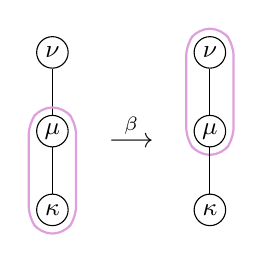
\begin{tikzpicture}
    \node (t3)[circle,draw=black,minimum size=4mm,inner sep=0.1mm] at (0,0) {\small $\kappa$};
    \node (t2) [circle,draw=black,minimum size=4mm,inner sep=0.1mm] at (0,1) {\small $\mu$};
    \node (t1) [circle,draw=black,minimum size=4mm,inner sep=0.1mm] at (0,2) {\small $\nu$};  
    \draw[-] (t3)--(t2) node {};
    \draw[-] (t2)--(t1) node {};
    \draw [Plum,rounded corners,thick] (-0.15+2,0.7) -- (-0.3+2,0.9) -- (-0.3+2,2.1) -- (-0.15+2,2.3) -- (0.15+2,2.3) -- (0.3+2,2.1) -- (0.3+2,0.9) -- (0.15+2,0.7) -- cycle;

    \node (B) at (1,1) {$\overset{\beta}{\longrightarrow}$};

    \node (b3)[circle,draw=black,minimum size=4mm,inner sep=0.1mm] at (2,0) {\small $\kappa$};
    \node (b2) [circle,draw=black,minimum size=4mm,inner sep=0.1mm] at (2,1) {\small $\mu$};
    \node (b1) [circle,draw=black,minimum size=4mm,inner sep=0.1mm] at (2,2) {\small $\nu$};  
    \draw[-] (b3)--(b2) node {};
    \draw[-] (b2)--(b1) node {};
    \draw [Plum,rounded corners,thick] (1.85-2,-0.3) -- (1.7-2,-.1) -- (1.7-2,1.1) -- (1.85-2,1.3) -- (2.15-2,1.3) -- (2.3-2,1.1) -- (2.3-2,-.1) -- (2.15-2,-.3) -- cycle;
\end{tikzpicture}} \quad\quad \raisebox{2.75em}{}\quad\quad 
\resizebox{0.4\linewidth}{!}{
\raisebox{1em}{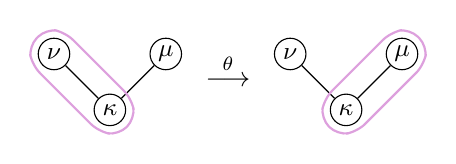
\begin{tikzpicture}
    \node (t3)[circle,draw=black,minimum size=4mm,inner sep=0.1mm] at (0,0) {\small $\kappa$};
    \node (t2) [circle,draw=black,minimum size=4mm,inner sep=0.1mm] at (0.71,0.71) {\small $\mu$};
    \node (t1) [circle,draw=black,minimum size=4mm,inner sep=0.1mm] at (-0.71,0.71) {\small $\nu$};  
    \draw[-] (t3)--(t1) node {};
    \draw[-] (t2)--(t3) node {};
    \draw [Plum,rounded corners,thick] (0.11,-0.32) -- (-0.14,-0.28) -- (-0.99,0.57) -- (-1.03,0.81) -- (-0.81,1.03) -- (-0.57,0.99)  -- (0.28,0.14) -- (0.32,-0.11) -- cycle;

    \node (B) at (1.5,0.5) {$\overset{\theta}{\longrightarrow}$};

    \node (b3)[circle,draw=black,minimum size=4mm,inner sep=0.1mm] at (3,0) {\small $\kappa$};
    \node (b2) [circle,draw=black,minimum size=4mm,inner sep=0.1mm] at (3+0.71,0.71) {\small $\mu$};
    \node (b1) [circle,draw=black,minimum size=4mm,inner sep=0.1mm] at (3-0.71,0.71) {\small $\nu$};  
    \draw[-] (b3)--(b1) node {};
    \draw[-] (b2)--(b3) node {};
    \draw [Plum,rounded corners,thick] (3-0.32,-0.11) -- (3-0.28,0.14) -- (3+0.57,0.99) -- (3+0.81,1.03) -- (3+1.03,0.81) -- (3+0.99,0.57) -- (3+0.14,-0.28) -- (3-0.11,-0.32) -- cycle;
\end{tikzpicture}}} \raisebox{2.75em}{} 
\end{center} 
\caption{The $\beta$ and $\theta$ isomorphisms defining a categorified non-symmetric operad.}
\label{fig:betatheta}
\end{figure}

\begin{figure}[h!]
\centering 
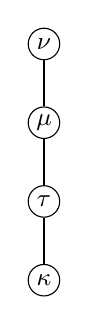
\begin{tikzpicture}
    \node (t3)[circle,draw=black,minimum size=4mm,inner sep=0.1mm] at (0,0) {\small $\kappa$};
    \node (t2) [circle,draw=black,minimum size=4mm,inner sep=0.1mm] at (0,1) {\small $\tau$};
    \node (t1) [circle,draw=black,minimum size=4mm,inner sep=0.1mm] at (0,2) {\small $\mu$};  
    \node (t4) [circle,draw=black,minimum size=4mm,inner sep=0.1mm] at (0,3) {\small $\nu$};  
    \draw[-] (t4)--(t1) node {};
    \draw[-] (t3)--(t2) node {};
    \draw[-] (t2)--(t1) node {};
\end{tikzpicture}
\quad \quad
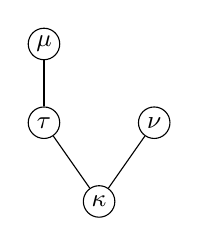
\begin{tikzpicture}
    \node (t3)[circle,draw=black,minimum size=4mm,inner sep=0.1mm] at (0,0) {\small $\kappa$};
    \node (t2) [circle,draw=black,minimum size=4mm,inner sep=0.1mm] at (-0.7,1) {\small $\tau$};
    \node (t1) [circle,draw=black,minimum size=4mm,inner sep=0.1mm] at (-0.7,2) {\small $\mu$};  
    \node (t4) [circle,draw=black,minimum size=4mm,inner sep=0.1mm] at (0.7,1) {\small $\nu$};  
    \draw[-] (t4)--(t3) node {};
    \draw[-] (t3)--(t2) node {};
    \draw[-] (t2)--(t1) node {};
\end{tikzpicture}
\quad \quad
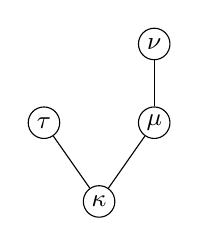
\begin{tikzpicture}
    \node (t3)[circle,draw=black,minimum size=4mm,inner sep=0.1mm] at (0,0) {\small $\kappa$};
    \node (t2) [circle,draw=black,minimum size=4mm,inner sep=0.1mm] at (-0.7,1) {\small $\tau$};
    \node (t1) [circle,draw=black,minimum size=4mm,inner sep=0.1mm] at (0.7,1) {\small $\mu$};  
    \node (t4) [circle,draw=black,minimum size=4mm,inner sep=0.1mm] at (0.7,2) {\small $\nu$};  
    \draw[-] (t4)--(t1) node {};
    \draw[-] (t3)--(t1) node {};
    \draw[-] (t2)--(t3) node {};
\end{tikzpicture}
\quad \quad
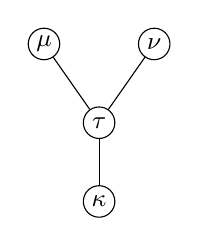
\begin{tikzpicture}
    \node (t3)[circle,draw=black,minimum size=4mm,inner sep=0.1mm] at (0,0) {\small $\kappa$};
    \node (t2) [circle,draw=black,minimum size=4mm,inner sep=0.1mm] at (0,1) {\small $\tau$};
    \node (t1) [circle,draw=black,minimum size=4mm,inner sep=0.1mm] at (-0.7,2) {\small $\mu$};  
    \node (t4) [circle,draw=black,minimum size=4mm,inner sep=0.1mm] at (0.7,2) {\small $\nu$};  
    \draw[-] (t4)--(t2) node {};
    \draw[-] (t3)--(t2) node {};
    \draw[-] (t2)--(t1) node {};
\end{tikzpicture}
\quad \quad
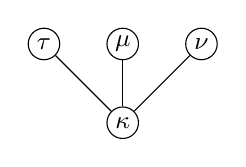
\begin{tikzpicture}
    \node (t3)[circle,draw=black,minimum size=4mm,inner sep=0.1mm] at (0,0) {\small $\kappa$};
    \node (t2) [circle,draw=black,minimum size=4mm,inner sep=0.1mm] at (-1,1) {\small $\tau$};
    \node (t1) [circle,draw=black,minimum size=4mm,inner sep=0.1mm] at (0,1) {\small $\mu$};  
    \node (t4) [circle,draw=black,minimum size=4mm,inner sep=0.1mm] at (1,1) {\small $\nu$};  
    \draw[-] (t4)--(t3) node {};
    \draw[-] (t3)--(t2) node {};
    \draw[-] (t3)--(t1) node {};
\end{tikzpicture}
\caption{The five planar trees with four vertices, giving rise to the pentagonal (first three) and hexagonal (last two) identites.}
\label{fig:planar4trees}
\end{figure}

\begin{rem}
\label{rem:DPLA}
K. Do{\v s}en and Z. Petri{\'c} introduced in \cite[Sec.~12]{DP15} the notion of weak Cat-operad.
Despite looking different at first sight, the two notions are in fact equivalent.
The crucial observation is the following: the $\theta$-isomorphisms of Do{\v s}en--Petri{\'c} comprise both the isomorphisms~$\theta$ in \cref{def:catoperad} and their inverses $\theta^{-1}$.
Therefore, there are only two pentagonal coherence diagrams in the definition of a weak Cat-operad, the equations ($\beta$ $pent_e$) and ($\beta\theta 2_e$) of \cite[Section 9]{DP15}.
The set of diagrams of the form ($\beta$ $pent_e$) is the same as the set of diagrams which arises from the first pentagon in \cref{def:catoperad}, while the set of diagrams of the form ($\beta\theta 2_e$) is partitioned into the sets of diagrams which arise from the second and third pentagons in \cref{def:catoperad}.

We will give in \cref{thm:coherence-operahedra} two topological proofs of coherence for categorified non-symmetric operads.
A benefit of our presentation is that, adopting the oriented approach (see the second proof of \cref{thm:coherence-operahedra}), we get a proof of coherence where $\beta$ and $\theta$ are both treated as rewriting rules, in contrast with the proof in \cite{DP15}, which proceeds in two stages: first get rid of $\beta$ (rewriting), then deal with $\theta$. 
See also \cref{rem:29}.
\end{rem}

\begin{definition}
    A \defn{strong morphism} of categorified non-symmetric operads $F: \mathcal{P} \to \mathcal{Q}$ is a collection of functors $F_n : \mathcal{P}(n) \to \mathcal{Q}(n)$ together with natural isomorphisms $$ \gamma_{\kappa,\mu}: F_{m-1+n}(\kappa \circ_i \mu) \overset{\cong}{\longrightarrow} F_m(\kappa) \circ_i F_n(\mu) $$ such that the following diagrams commute:
    \begin{center}
    \resizebox{\linewidth}{!}{
    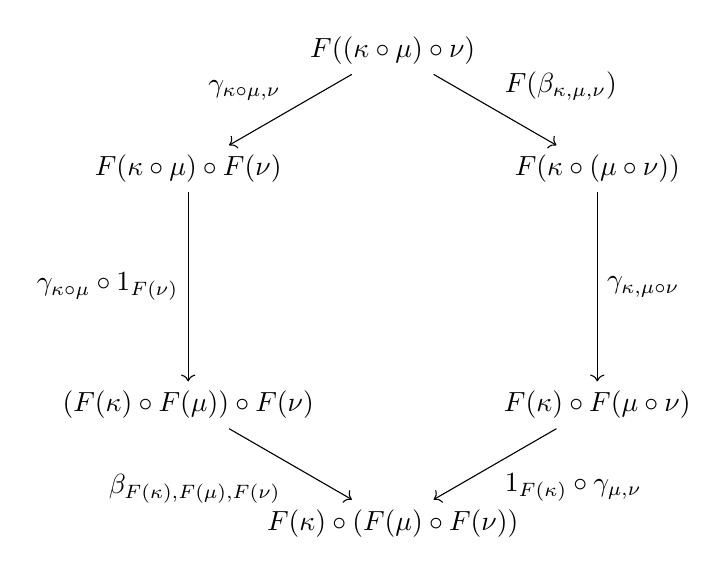
\begin{tikzpicture}[scale=3]
        \node (P1) at (0,1) {$F((\kappa\circ\mu)\circ\nu)$};
        \node (P2) at (-0.866,0.5) {$F(\kappa\circ\mu)\circ F(\nu)$};
        \node (P3) at (-0.866,-0.5) {$(F(\kappa)\circ F(\mu))\circ F(\nu)$};
        \node (P4) at (0,-1) {$F(\kappa)\circ(F(\mu)\circ F(\nu))$};
        \node (P5) at (0.866,0.5) {$F(\kappa\circ(\mu\circ\nu))$} ;
        \node (P6) at (0.866,-0.5) {$F(\kappa)\circ F(\mu\circ\nu)$};
        \draw[->] (P1)--(P2) node[midway,above left] {$\gamma_{\kappa\circ\mu,\nu}$};
        \draw[->] (P2)--(P3) node[midway,left] {$\gamma_{\kappa\circ\mu}\circ 1_{F(\nu)}$};
        \draw[->] (P3)--(P4) node[midway,below left] {$\beta_{F(\kappa),F(\mu),F(\nu)}$};
        \draw[->] (P1)--(P5) node[midway,above right] {$F(\beta_{\kappa,\mu,\nu})$};
        \draw[->] (P5)--(P6) node[midway,right] {$\gamma_{\kappa,\mu\circ\nu}$};
        \draw[->] (P6)--(P4) node[midway,below right] {$1_{F(\kappa)}\circ\gamma_{\mu,\nu}$};
    \end{tikzpicture}  \quad \quad
    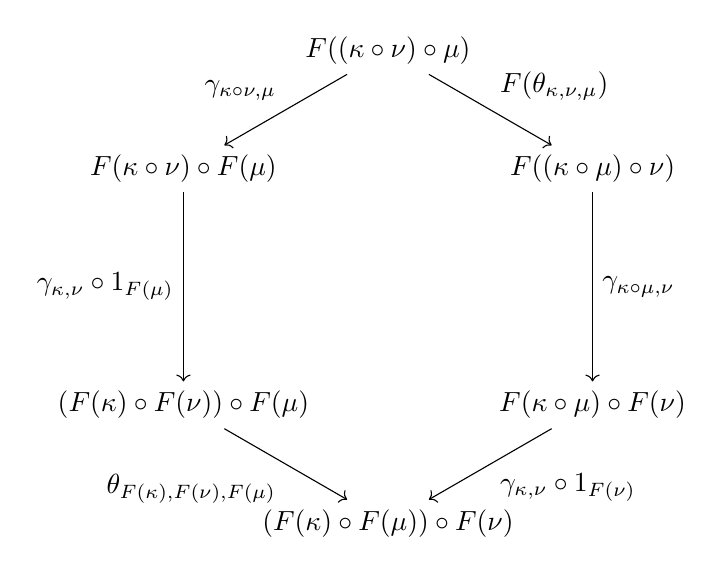
\begin{tikzpicture}[scale=3]
        \node (P1) at (0,1) {$F((\kappa\circ\nu)\circ\mu)$};
        \node (P2) at (-0.866,0.5) {$F(\kappa\circ\nu)\circ F(\mu)$};
        \node (P3) at (-0.866,-0.5) {$(F(\kappa)\circ F(\nu))\circ F(\mu)$};
        \node (P4) at (0,-1) {$(F(\kappa)\circ F(\mu))\circ F(\nu)$};
        \node (P5) at (0.866,0.5) {$F((\kappa\circ\mu)\circ\nu)$} ;
        \node (P6) at (0.866,-0.5) {$F(\kappa\circ\mu)\circ F(\nu)$};
        \draw[->] (P1)--(P2) node[midway,above left] {$\gamma_{\kappa\circ\nu,\mu}$};
        \draw[->] (P2)--(P3) node[midway,left] {$\gamma_{\kappa,\nu}\circ 1_{F(\mu)}$};
        \draw[->] (P3)--(P4) node[midway,below left] {$\theta_{F(\kappa),F(\nu),F(\mu)}$};
        \draw[->] (P1)--(P5) node[midway,above right] {$F(\theta_{\kappa,\nu,\mu})$};
        \draw[->] (P5)--(P6) node[midway,right] {$\gamma_{\kappa\circ\mu,\nu}$};
        \draw[->] (P6)--(P4) node[midway,below right] {$\gamma_{\kappa,\nu}\circ 1_{F(\nu)}$};
    \end{tikzpicture}  } \quad \ .
\end{center}
    It is said to be \defn{strict} if the natural isomorphisms are identities. 
\end{definition}

Once again, the diagrams above hold for all instances of $\beta$ and $\theta$ arrows, and we have omitted the $(i,j,k)$-indices for readability. 
Observe that a strong (resp. strict) morphism between categorified non-symmetric operads concentrated in arity $1$ is a strong (resp. strict) monoidal functor between non-symmetric monoidal categories. 

%%%%%%%%%%%%%%%%%%%%%%%%%%%%%%%%%%%%%%%%%%%%%%%

\subsection{Coherence theorem}

We now aim at the coherence theorem for categorified non-symmetric operads.
In order to state the theorem, we construct the free non-symmetric categorified operad on a family of sets $S=\{S_n\}_{n \geq 1}$.
We define a family of categories $\mathcal{S}=\{\mathcal{S}_n\}_{n \geq 1}$ whose objects are given by the following rules:
\begin{enumerate}
    \item if $\mu \in S_n$, then $\mu$ is an object of $\mathcal{S}_n$;
    \item if $\mu \in \mathcal{S}_m$ and $\nu \in \mathcal{S}_n$, then $\mu \circ_i \nu$ is an object of $\mathcal{S}_{m-1+n}$, for any $1 \leq i \leq m$.
\end{enumerate}
If an object $\mu$ is in $\mathcal{S}_n$, we say that $\mu$ has \defn{arity} $n$. 
Now we define a set $M$ of basic morphisms $\beta: (\kappa \circ_i \mu) \circ_{j+i-1} \nu \leftrightarrow \kappa \circ_i (\mu \circ_j \nu) : \beta^{-1}$ for every $\kappa \in \mathcal{S}_m, \mu \in \mathcal{S}_n, \nu \in \mathcal{S}_k$, $1 \leq i \leq m$ and $1 \leq j \leq n$, and $\theta: (\kappa \circ_i \nu) \circ_{j-1+k} \mu \leftrightarrow (\kappa \circ_j \mu) \circ_i \nu : \theta^{-1}$ whenever $i<j$.
We then define the generating morphisms of the family $\mathcal{S}$ by the following rules:
\begin{enumerate}
    \item if $\phi \in M$, then $\phi$ is a generating morphism of $\mathcal{S}$; 
    \item if $\phi : t_1 \to t_2$ is a generating morphism in $\mathcal{S}$, and $t_3 \in \mathcal{S}$, then $\phi \circ_i \id : t_1 \circ_i t_3 \to t_2 \circ_i t_3$ and $\id \circ_j \phi : t_3 \circ_j t_1 \to t_3 \circ_j t_2$ are morphisms, for any $i$ (resp. $j$) between $1$ and the arity of $t_1$ (resp. $t_3$).
\end{enumerate}
Note that by construction, for every morphism $\phi : t_1 \to t_2$, the objects $t_1$ and $t_2$ have the same arity, and we say that $\phi$ has this \defn{arity}. 
We then define $\mathcal{S}_n$ as the free category over all generating morphisms of arity $n$. 
This finishes the construction of our family $\mathcal{S}$ of categories.

\begin{definition}
    We denote by $\mathcal{F}(S)$ the quotient of the family of categories $\mathcal{S}$ by localization (inverting the $\beta$ and $\theta$ morphisms), the axioms of bifunctors, and the coherence diagrams defining a categorified non-symmetric operad. 
\end{definition}

We obtain that $\mathcal{F}(S)$ is the free categorified non-symmetric operad on $S$. 
That is, for any categorified non-symmetric operad $\mathcal{P}$, and for any family of functions $\rho_n : S_n \to \obj(\mathcal{P}(n))$, there is a unique \emph{strict} morphism of non-symmetric categorified operads $\mathcal{F}(S) \to \mathcal{P}$ which extends $\rho=\{\rho_n\}_{n\geq 1}$. 
By precomposing it with the quotient map $\mathcal{S} \to \mathcal{F}(S)$, we get a levelwise functor $[-]:\mathcal{S} \to \mathcal{P}$.

\begin{thm}[Coherence theorem]
\label{thm:coherence-operahedra}
    For any categorified non-symmetric operad $\mathcal{P}$, for any family of functions $\rho : S \to \obj(\mathcal{P})$, and for any two parallel morphisms $\phi_1,\phi_2: t_1 \to t_2$ in~$\mathcal{S}$, we have $[\phi_1]=[\phi_2]$.
\end{thm}

\correction{
In order to prove this Theorem, we need to first recall from \cite[Sec.~2.1]{laplante-anfossiDiagonalOperahedra2022a}, see also \cite[Sec.~13]{DP15} and \cite{curienSyntacticAspectsHypergraph2019a} the construction of the operahedra, a family of polytopes whose faces are in bijection with the set of all nestings on a planar tree.
\begin{proposition}
    There are bijections between
    \begin{itemize}
        \item objects of $\calS$ and vertices 
        \item generating morphisms and edges
        \item coherence, bifunctoriality and naturality diagrams and $2$-faces
    \end{itemize}
\end{proposition}
\begin{proof}
    One can think about the objects of $\mathcal{S}$ as the set of fully nested planar trees whose vertices are decorated by objects of $S$, subject to the requirement that if a vertex has $n$ incoming edges, it must be decorated by an element of $S_n$. 
The nests in the tree represent the order in which the objects decorating the vertices should be formally composed, as represented in \cref{fig:treeandnesting}.
Morphisms in $\mathcal{S}$ are sequences of applications of the associativity rules~$\beta$ and~$\theta$, moving one nest at a time to a neighbouring pair of vertices as in \cref{fig:betatheta}.
\end{proof}
then}

\begin{proof}
The morphisms of $\mathcal{S}$ are in bijection with combinatorial paths on a family of polytopes called operahedra \cite[Sec.~2.1]{laplante-anfossiDiagonalOperahedra2022a}, see also \cite[Sec.~13]{DP15} and \cite{curienSyntacticAspectsHypergraph2019a}, whose faces are in bijection with the set of all nestings on a planar tree. 
There is one operahedron for each planar tree $t$, and its vertices are in bijection with the maximal (full) nestings of~$t$ and edges between them are in bijection with the generating morphisms between the corresponding terms. 
Two parallel morphisms in $\mathcal{S}$ thus define two parallel combinatorial paths on some operahedron. 
Since an operahedron is simply connected, \cref{thm:top-coherence} implies that these two combinatorial paths are combinatorially homotopic. 
The result then follows from the fact that a $2$-face of an operahedron is exactly either a square (witnessing naturality), a pentagon or an hexagon (witnessing a coherence condition) as in \cref{def:catoperad} above.
\end{proof}

\begin{proof}[Second proof]
    Alternatively, since the operahedra are polytopes, one can use \cref{prop:polytopes} and \cref{p:second-proof}. 
    Choosing a generic vector $\vec v$ which has strictly decreasing coordinates for the Loday realizations \cite[Section 2.2]{laplante-anfossiDiagonalOperahedra2022a} gives the orientations of the diagrams given in \cref{def:catoperad} on every $2$-face \cite[Proposition 3.11]{laplante-anfossiDiagonalOperahedra2022a}.
    The posets/rewriting system obtained generalize the Tamari lattice on fully nested linear trees \cite[Definition 2.8]{laplante-anfossiDiagonalOperahedra2022a}.
    One then obtains a topological proof of coherence which is almost word for word the original proof of MacLane \cite[Theorem 3.1]{MacLane63}, suitably generalized to categorified operads. 
\end{proof}
   
Following \cref{rem:DPLA}, we have that \cref{thm:coherence-operahedra} gives an alternative, more economical proof of coherence for weak Cat-operads \cite[Proposition 14.2]{DP15}.
Incidentally, it gives an alternative input to the proof of coherence for cyclic symmetric categorified operads \cite{curienCategorifiedCyclicOperads2020}.

Restricting the theorem above to non-symmetric operads concentrated in arity $1$, the category $\mathcal{F}(S)$ becomes the free non-symmetric monoidal category on $S$, and we get the following corollary. 

\begin{corollary}[MacLane's coherence theorem for non-symmetric monoidal categories]
\label{cor:MacLane}
    For any non-symmetric monoidal category $\mathcal{C}$, for any function $\rho : S \to \obj(\mathcal{C})$, and for any two parallel morphisms $\phi_1,\phi_2: t_1 \to t_2$ in $\mathcal{S}$, we have $[\phi_1]=[\phi_2]$.
\end{corollary}

%%%%%%%%%%%%%%%%%%%%%%%%%%%%%%%%%%%%%

\subsection{Symmetric monoidal categories} 
One can use the same ideas to prove MacLane's coherence theorem for \emph{symmetric} monoidal categories, using the family of permutoassociahedra \cite{kapranov1993,reinerCoxeterassociahedra1994,baralicSimplePermutoassociahedron2019,CastilloLiu21}. 
Here we simply formulate the theorem, the proof is really the same as the one of \cref{thm:coherence-operahedra}.

Let $W_n$ denote the set of non-commutative, fully parenthesized words on $n$ distinct letters. 
Let $(\mathcal{C}, \otimes)$ be a symmetric monoidal category.
Each $w \in W_n$ defines in an obvious way a functor $[w] : \mathcal{C}^{\times n} \to \mathcal{C}$.
For instance, if $w=((ab)c)(ed)$, then the associated functor is defined on objects and morphisms by the formula
\begin{eqnarray*}
    [w] \quad : \quad \mathcal{C}^{\times n} & \to & \mathcal{C} \\
    (a,b,c,d,e) & \mapsto & ((a \otimes b) \otimes c)\otimes (e \otimes d) \ .
\end{eqnarray*}
We consider the free category $\mathcal{W}_n$ which has objects the elements of $W_n$, and morphisms generated by the ones of the form $\phi : w_1 \to w_2$, where the word $w_2$ is obtained from $w_1$ by applying either $\alpha : ((ww')w'') \to (w(w'w''))$, $\alpha^{-1}$, or $\tau : ww' \to w'w$ to a subword of $w_1$.
To any such $\phi$ one can associate a natural transformation $[\phi] : [w_1] \to [w_2]$ in $\mathcal{C}$ in the obvious way. 

\begin{thm}[MacLane's coherence theorem]
    \label{thm:MacLane}
    For any symmetric monoidal category $\mathcal{C}$, and for any pair of parallel morphisms $\phi_1,\phi_2: w_1 \to w_2$ in $\mathcal{W}=\{\mathcal{W}_n\}_{n\geq 1}$, we have $[\phi_1]=[\phi_2]$.
\end{thm}

%%%%%%%%%%%%%%%%%%%%%%%%%%%%%%%%%%%%%

\subsection{Rewriting perspective}

\correction{make this a paragraph}
\begin{rem}
    In the tree representation for $\mathcal{S}$, there is a coherence diagram for every decorated planar tree with 4 vertices, see \cref{fig:planar4trees}.
    In the rewriting system formed by the fully nested planar trees and the $\beta$ and $\theta$ arrows, these correspond precisely to the critical pairs \cite[Section 6.2]{baaderTermRewritingAll1998}.
\end{rem}

\begin{rem}
\label{rem:29}
MacLane's original proof \cite{MacLane63} proceeds in two stages, (anachronically) much like the one of Do{\v s}en--Petri{\'c} for weak Cat-operads (\cref{rem:DPLA}).
But the second proof of \cref{thm:coherence-operahedra} suggests a one stage proof: indeed, fixing a total order on the letters, allowing $\tau: ab \to ba$ only if the maximal letter is in $a$ (and adding $\tau^{-1}$), we get a terminating and confluent rewriting system. 
\end{rem}

%%%%%%%%%%%%%%%%%%%%%%%%%%%%%%%%%%%%%

\subsection{Further applications} 
\label{sec:further}
One can also use the same strategy to prove coherence for \emph{unital} non-symmetric monoidal categories, using the unital associahedra of F. Muro and A. Tonks \cite{muroUnitalAssociahedra2014}.

It is natural to ask if the construction of unital associahedra could be extended to the permutoassociahedra, in such a way as to provide a topological proof of coherence for unital symmetric monoidal categories. 
The question of the existence of these constructions at the operadic level (i.e. does there exist unital operahedra, symmetric operahedra, and unital symmetric operahedra?) is, to our knowledge, still open as well. 

Another immediate application of \cref{thm:top-coherence} is the coherence of strong non-symmetric monoidal functors between non-symmetric monoidal categories \cite{epsteinFunctorsTensoredCategories1966}. 
The corresponding topological objects are in this case the family of multiplihedra \cite{Stasheff70,Forcey08}.
The generalization to strong morphisms between non-symmetric categorified operads also goes through, involving this time the family of multiploperahedra described at the end of the introduction in \cite{MazuirLA22}.

In the same spirit as in \cref{thm:coherence-operahedra}, one could obtain coherence results for categorifications of many operad-like structures, for instance the ones described in \cite{BMO20}: categorified modular operads, wheeled properads, and permutads (shuffle algebras), among others.
In order to treat cyclic and symmetric structures, one could take inspiration from the reduction process followed in \cite{curienCategorifiedCyclicOperads2020} for the case of cyclic symmetric categorified operads.


% !TEX root = ../Coherence.tex

\section{Perspectives}

%%%%%%%%%%%%%%%%%%%%%%%%%%%%%%%%%%%%%

\subsection{Further applications} 
\label{sec:further}
One can also use the same strategy to prove coherence for \emph{unital} non-symmetric monoidal categories, using the unital associahedra of F. Muro and A. Tonks \cite{muroUnitalAssociahedra2014}.

It is natural to ask if the construction of unital associahedra could be extended to the permutoassociahedra, in such a way as to provide a topological proof of coherence for unital symmetric monoidal categories. 
The question of the existence of these constructions at the operadic level (i.e. does there exist unital operahedra, symmetric operahedra, and unital symmetric operahedra?) is, to our knowledge, still open as well. 

Another immediate application of \cref{thm:top-coherence} is the coherence of strong non-symmetric monoidal functors between non-symmetric monoidal categories \cite{epsteinFunctorsTensoredCategories1966}. 
The corresponding topological objects are in this case the family of multiplihedra \cite{Stasheff70,Forcey08}.
The generalization to strong morphisms between non-symmetric categorified operads also goes through, involving this time the family of multiploperahedra described at the end of the introduction in \cite{MazuirLA22}.

In the same spirit as in \cref{thm:coherence-operahedra}, one could obtain coherence results for categorifications of many operad-like structures, for instance the ones described in \cite{BMO20}: categorified modular operads, wheeled properads, and permutads (shuffle algebras), among others.
In order to treat cyclic and symmetric structures, one could take inspiration from the reduction process followed in \cite{curienCategorifiedCyclicOperads2020} for the case of cyclic symmetric categorified operads.

\subsection{Higher categories} 
\label{sec:higher}
\cref{thm:top-coherence} demonstrates that, in the case of monoidal categories, coherence is equivalent to the vanishing of the first homotopy groups of the associahedra. 
Since the associahedra are contractible, and therefore all their homotopy groups vanish, one could hope for a topological proof of higher dimensional coherence theorems.
Seeing a monoidal category as a bicategory with one object, one can ask about a coherence theorem for tricategories with one object. 
A first look at the diagrams in the beginning of \cite[Section 2]{gordonCoherenceTricategories1995} suggests that such a theorem should be at least related to the vanishing of the second homotopy groups of the associahedra.  
To formulate higher dimensional statements, one needs a good structure of pasting scheme on each associahedron, which is the subject of ongoing work \cite{AMMLA}. 

Recent results of S. Barkan provide evidence for these higher dimensional statements, in the context of $\infty$-operads \cite{barkanArityApproximationInfty2022}.
In this vein, it seems likely that the present results could be interpreted as a strict version and a special case of \cite[Theorem B]{barkanArityApproximationInfty2022}. 
It would be interesting to see how the permutoassociahedra arise in the strictification process, and how they are related to operadic partition complexes.  

\correction{Add Kapranov--Voevodsky one dimension higher; autre reference ou la correspondance semble etre faite}




%% !TEX root = ../Coherence.tex

\section{Koszulity via rewriting} 
\label{s:rewriting}


Let us take a detour by the Koszul duality theory for operads. One of the standard method for proving that an operad is Koszul is the "rewriting method" \cite[Section 8.3]{LodayVallette12}. The generalization to the colored case was done recently by V. Kharitonov and A. Khoroshkin \cite[Theorem 3.12]{KhariKhoro20}.

\begin{thm}[Rewriting method for colored operads {\cite[Theorem 8.3.1]{LodayVallette12}}] \label{thm:rewriting} Let $\mathcal{O}(E,R)$ be a quadratic colored operad. If its generating space $E$ admits a $\mathbb{K}$-linear ordered basis, for which there exists a suitable order on shuffle trees, such that every critical monomial is confluent then the colored operad $\mathcal{O}$ is Koszul. 
\end{thm}

In this case, the operad $\mathcal{O}$ admits an induced shuffle tree basis sharing nice properties, called a PBW basis, see \cite[Section 8.5.3]{LodayVallette12}. Parler Grobner Basis

\begin{thm} \label{thm:Koszulrewriting} The colored operad $\mathcal{O}$ is a Koszul colored operad. 
\end{thm}
\begin{proof} The partial order on complete nested trees defined in X induces, via the proof of X, a suitable order on shuffle trees, see X. The 1-skeleton of operahedra appears as the application of the rewriting rules given by the sequential and parallel axioms. We consider the family of trees $F=\{\tau \in \mathrm{OT}=\ | \ |V(\tau)|=4\}$ and the oriented operahedra $\{(P_\tau,\vec v)\}_{\tau \in F}$ for any vector $\vec v=(v_1,v_2,v_3)$ such that $v_1>v_2>v_3$. Every critical monomial corresponds to the complete nested trees associated to $\{bot(P_\tau,\vec v)\}_{\tau \in F}$, and X implies that every critical monomial is confluent. We conclude by \cref{thm:rewriting}. 
The complete nested trees associated to $\{top(P_\tau, \vec v)\}_{\tau \in F}$ form the PBW basis of $\mathcal{O}_{ns}$.
\end{proof}

The proof of \cref{thm:rewriting} relies on the Diamond Lemma \cite[Theorem 8.5.5]{LodayVallette12}. Instead, we can use the full power of X.

\begin{proof}[Second proof] Every rewriting diagram associated to a monomial is part of the 1-skeleton of some operahedron of dimension $n\geq 0$. By X, this 1-skeleton is oriented and forms the boundary of a topological $n$-ball. Thus, it has a unique maximal element. 
\end{proof}

Restricting to linear trees, we have that the operad $\mathrm{Ass}$ is Koszul. Restricting to the 2-leveled trees as in X, we obtain that the permutad $\mathrm{permAs}^h$ is Koszul, in the sense of M. Markl \cite[Definition 21]{Markl19}.

\medskip

\cref{thm:Koszulrewriting} gives an alternative proof of \cref{thm:coherence}. 

\begin{proof}[Second proof of {\cref{thm:coherence}}] Let $\mathcal{O}$ be a non-unital categorified ns operad. The pentagonal and hexagonal diagrams commute, and they correspond precisely to the 1-skeleton of the 2-dimensional oriented operahedra $\{(P_\tau,\vec v)\}_{\tau \in F}$. Using the Diamond Lemma as in the proof of \cref{thm:rewriting}, we have that every diagram made up of $\theta$ and $\beta$ arrows commute. 
\end{proof}

Here again, resorting to the Diamond Lemma is not necessary.

\begin{proof}[Third proof of {\cref{thm:coherence}}] Any diagram $D$ made up of $\theta$ and $\beta$ arrows lives on the 1-skeleton of an operahedron of some dimension $n\geq 0$. As this operahedron is topologically a $n$-dimensional ball, the diagram $D$ is obtained by gluing together 1-skeletons of 2-dimensional operahedra, which commute by hypothesis.
\end{proof}

As noted in \cite[Remark p.266]{LodayVallette12} for MacLane's coherence theorem, the proofs of the Koszulity of $\mathcal{O}$ and of the coherence theorem are formally the same, and both can be given "instant one-step proofs" via the underlying polytopes. This suggests a common ground for both statements [Maxime Lucas?].
%% !TEX root = ../Coherence.tex

\section{Koszul duality} 
\label{s:koszul}



Another standard method to prove that an operad is Koszul is the "operadic partition poset method" \cite[Section 8.7]{LodayVallette12}. Its extension to the colored setting is straightforward.

\begin{thm}[Koszul-Cohen-Macaulay criterion {\cite[Theorem 8.7.5]{LodayVallette12}}] \label{thm:koszulmacaulay} Let $\mathrm{O}$ be a quadratic basic-set $X$-colored operad generated by a homogeneous $\mathbb{S}$-set concentrated in arity $k$, with $k\geq 2$. Let $\Pi_{\mathrm{O}}(x_1,\ldots,x_n;x_0)$ denote the colored operadic partition posets.
\begin{itemize}
    \item The linear colored operad $\calO=\KK\mathrm{O}$ is a Koszul colored operad if and only if, for every $n\geq 1$ and every $\omega \in \mathrm{Max}(\Pi_{\mathrm{O}}(x_1,\ldots,x_n;x_0))$, the interval $[\hat 0,\omega]$ is Cohen-Macaulay. 
    \item The top homology groups are isomorphic to the Koszul dual cooperad \[H_{\mathrm{top}}(\Pi_{\mathrm{O}}(x_1,\ldots,x_n;x_0))\cong \calO^{\as}(x_1,\ldots,x_n;x_0) \]
\end{itemize}
\end{thm}

%We can apply this theorem to the operad $\calO_{ns}$ to obtain an alternative proof of \cref{thm:Koszulrewriting}.

\begin{proof}[{\cref{thm:Koszulrewriting}}, third proof] The operad $\calO_{ns}$ is a quadratic basic-set $\mathbb{N}$-colored operad generated by a homogeneous $\mathbb{S}$-set concentrated in arity 2. A colored operadic partition poset $\Pi_{\mathrm{OT}}(x_1,\ldots,x_n;x_0)$ is the poset of nestings of all the possible operadic trees obtained by grafting $n$ corollas with $x_1,\ldots,x_n$ leaves and respecting the planar canonical numbering. A maximal element $\omega$ in $\Pi_{\mathrm{OT}}(x_1,\ldots,x_n;x_0)$ is a particular operadic tree $\tau \in \mathrm{OT}$ with $n$ vertices, and an interval $[\hat 0,\omega]$ is the poset of nestings $\mathrm{N}_\tau$ of $\tau$. This poset is a lattice, thus it is also Cohen-Macaulay. 
\end{proof}

So we see that the posets $[\hat 0,\omega]$ have more structure than the Cohen-Macaulay property, which is a condition equivalent to Koszulity. They are lattices, moreover isomorphic to face lattices of polytopes. This suggests that the operad $\calO_{ns}$ has further algebraic properties. 



\begin{thm} \label{prop:koszulpoincare} Let $\mathrm{O}$ be a quadratic set $X$-colored operad which is also finite in each arity, and let $\calO=\KK \mathrm{O}$ be its algebraic avatar. We suppose that there exists a family $P=\{P_\tau\}_{\tau \in \mathrm{O}}$ of polytopes inedexed by the elements of $\mathrm{O}$, which is endowed with a topological colored operad structure and such that we have an isomorphism of de colored cooperads (resp. operads) \[C^{-\bullet}_{\mathrm{cell}}(P)\cong B\calO \quad (\text{resp.} \ C_{\bullet}^{\mathrm{cell}}(P)\cong \Omega\calO^{\as})\ . \] Then, we have that
    \begin{enumerate}
        \item the colored operad $\calO$ is Koszul, 
        \item the colored operad $\calO$ is self-dual for Koszul duality, 
        \item there is an isomorphism of colored operads (resp. cooperads)  $C_{\bullet}^{\mathrm{cell}}(P)\cong \Omega\calO^{\as} \ (\text{resp.} C^{-\bullet}_{\mathrm{cell}}(P)\cong B\calO)$, and
        \item there is an isomorphism of colored operads $\Omega B \calO \cong C_{\bullet}^{\mathrm{cell}}(P_\mathrm{sub})$\ .
    \end{enumerate} 
\end{thm}
Here, $P_\mathrm{sub}$ stands for the family of polytopes $\{P_\tau^{\mathrm{sub}}\}_{\tau \in \mathrm{O}}$ where each polytope $P_\tau$ is endowed with its dual subdivision.
\begin{proof} 

\leavevmode
    
\begin{enumerate}
    \item The fact that the polytopes are contractible imply that the cohomology (resp. homology) of the bar (resp. cobar) construction is concentrated in syzygy degree zero.
    \item As $\calO$ comes from a set-theoretic colored operad, we have the following isomorphisms of dg colored cooperad 
    \begin{eqnarray*} 
        \calO^{\as}\cong H^{[\bullet]}(B\calO)
        = \bigoplus_{\tau \in \mathrm{O}} H^{[\dim P_\tau-\bullet]}\left(C^{\dim P_\tau -\bullet}_{\mathrm{cell}}(P_\tau)\right)\cong \bigoplus_{\tau \in \mathrm{O}} \KK \cong \calO^{*} \ . 
    \end{eqnarray*} 
    The symmetric statement is obtained by dualization.
    \item The preceding two points now imply the following chain of isomorphims of dg colored operads 
    \[\Omega \mathcal{O}^{\as} \cong (B(\mathcal{O}^{\as})^{*})^{*} \cong (B\mathcal{O}^{!})^{*}\cong (B\mathcal{O})^{*}\cong C_{\mathrm{cell}}^{-\bullet}(P)^{*} \cong C_\bullet^{\mathrm{cell}}(P)  \ . \] 
    \item \Guillaume{TBC}
\end{enumerate}
\end{proof}

\Guillaume{
\begin{itemize}
    \item Remonter au poset des compositions? (--> Giraudo)
    \item Rel\^acher les hypoth\`eses permet-t-il d'appliquer le r\'esultat de Jovana?
    \item Qu'arrive-t-il si on ne demande pas des polytopes mais seulement des CWCX?
\end{itemize}}




On a aussi gratuitement l'analogue de la proposition 9.3.2 du Loday-Vallette. 

%l'orientation compte
%structure d'opérade sur les polytopes abstraits


\begin{thm} \label{thm:OnsKoszul} The colored operad $\calO_{ns}$ is Koszul and self-dual. Moreover, the cellular chains [...].
\end{thm}
\begin{proof} \Guillaume{TBC}
\end{proof}


It seems likely that this theorem can be extended to other known operads governed by a colored operad: Suppose that $\mathcal{P}$ comes from a family of connected simple graphs with substitution. Then, $\mathcal{P}$ is Koszul self-dual and its minimal model is given by the cellular chains on a family of polytopes. 
\begin{proof}[Idea of proof] The bar construction on $\mathcal{P}$ corresponds to the nestings of the underlying graphs. Using the line graphs duality of Proposition \ref{proplinegraph} these can be realized by graph-associahedra. The cellular chains on this family of polytopes then gives us the minimal model $\Omega \mathcal{P}^{\as}$ of $\mathcal{P}$.
\end{proof} 
Some recent work go towards this direction. For instance: 
-constructs in J. Obradovi\'c, P.-L. Curien and J. Ivanovi\'c in \cite{CIO18}.
-minimal model in  J. Obradovi\'c in \cite{Obradovic19} 
-minimal models in  J. Obradovi\'c, M. Markl and M. Batanin in \cite{BMO20}
-and the work of Ward
-V-infinity dioperad
-Pilaud--LA dioperad
-Paul Laubie




%% !TEX root = ../Coherence.tex

\section{Poincar\'e duality} 
\label{s:poincare}


The Poincar\'e isomorphism between chains and cochains is precisely here the isomorphism establishing Koszul self-duality. This is particularly apparent from the last isomorphism $\Omega B \calO \cong C_{\bullet}^{\mathrm{cell}}(P_\mathrm{sub})$.

The intersection pairing gives the equivalence between the resolution and the operad. 

-Link with Salvatore--Ching for $E_n$


\bigskip

\emph{Acknowledgements.}   
We would like to thank all the participants of the Roberta Seminar held on September 30th, 2020 in Paris for planting the seeds of the present note.  
We would like to thank Andrea Bianchi for enlightening discussions, for pointing out mistakes in a first draft, and for reminding us of the Seifert--Van Kampen theorem. 
Finally, we are grateful to Zoran Petri{\'c} for precious discussions on weak Cat-operads.

\bibliographystyle{amsalpha}

\bibliography{Coherence}


\end{document}



